\documentclass[lettersize,journal]{IEEEtran}
\usepackage{amsmath,amsfonts}
\usepackage{algorithmic}
\usepackage{algorithm}
\usepackage{array}
\usepackage[caption=false,font=normalsize,labelfont=sf,textfont=sf]{subfig}
% \usepackage{caption}
\usepackage{textcomp}
\usepackage{stfloats}
\usepackage{url}
\usepackage{verbatim}
\usepackage{graphicx}
\usepackage{cite}
\usepackage{amssymb}
\usepackage{xcolor}
\usepackage{epsfig}
\usepackage{epstopdf} 
\usepackage{multirow}
% \usepackage[font={small}]{caption}
% \usepackage{caption}
% \usepackage[font=small]{caption}
\hyphenation{op-tical net-works semi-conduc-tor IEEE-Xplore}
% updated with editorial comments 8/9/2021

\begin{document}

\title{Sequential Task Assignment and Resource Allocation in V2X-Enabled Mobile Edge Computing}

\author{Yufei Ye, Shijian Gao,~\IEEEmembership{Member,~IEEE}, Xinhu Zheng,~\IEEEmembership{Member,~IEEE}, and Liuqing Yang,~\IEEEmembership{Fellow,~IEEE}
        % <-this % stops a space
% \thanks{The review of this article was coordinated by Prof. Shijian Gao. (Corresponding Author: Prof. Shijian Gao.)}% <-this % stops a space
% \thanks{Yufei Ye and Xinhu Zheng are with the Intelligent Transportation Thrust, The Hong Kong University of Science and Technology (Guangzhou), Guangzhou 511458, China (e-mail: yye760@connect.hkust-gz.edu.cn; xinhuzheng@hkust-gz.edu.cn).}
% \thanks{Shijian Gao is with the Internet of Things Thrust, The Hong Kong University of Science and Technology (Guangzhou), Guangzhou 511458, China (e-mail: shijiangao@hkust-gz.edu.cn).}
% \thanks{Liuqing Yang is with the Internet of Things Thrust and Intelligent Transportation Thrust, The Hong Kong University of Science and Technology
% (Guangzhou), Guangzhou 511458, China, and also with the Department of
% Electronic and Computer Engineering, The Hong Kong University of Science
% and Technology, Hong Kong SAR, China (e-mail: lqyang@ust.hk).}
}

% The paper headers
% \markboth{IEEE Transactions on Vehicular Technology,~Vol.~1, No.~1, March~2025}%
% {Shell \MakeLowercase{\textit{et al.}}: A Sample Article Using IEEEtran.cls for IEEE Journals}

% \IEEEpubid{0000--0000/00\$00.00~\copyright~2024 IEEE}
% Remember, if you use this you must call \IEEEpubidadjcol in the second
% column for its text to clear the IEEEpubid mark.

\maketitle


\begin{abstract}
Nowadays, the convergence of Mobile Edge Computing (MEC) and vehicular networks has emerged as a vital facilitator for the ever-increasing intelligent onboard applications. This paper introduces a multi-tier task offloading mechanism for MEC-enabled vehicular networks leveraging vehicle-to-everything (V2X) communications. The study focuses on applications with sequential subtasks and explores two tiers of collaboration. In the vehicle tier, we design a needing vehicle (NV)-helping vehicle (HV) matching scheme and inter-vehicle collaborative computation is studied, with joint optimization of task offloading decision, communication, and computation resource allocation to minimize energy consumption and meet latency requirements. In the roadside unit (RSU) tier, collaboration among RSUs is investigated to address multi-access issues of bandwidth and computation resources for multiple vehicles. A two-step method is proposed to solve the subchannel allocation problem. Detailed experiments are conducted to demonstrate the effectiveness of the proposed method and assess the impact of different parameters on system energy consumption.
\end{abstract}

\begin{IEEEkeywords}
Mobile edge computing (MEC), task offloading, vehicle-to-everything (V2X) communications, multi-access, sequential dependency, vehicular networks.
\end{IEEEkeywords}

\section{Introduction}
\IEEEPARstart{I}{n} recent years, significant advancements in intelligent vehicles \cite{ref1}, vehicular networks \cite{ref2,ref3}, and autonomous driving \cite{ref4} have greatly improved safety, efficiency, and comfort for both drivers and passengers \cite{ref5}. Utilizing advanced sensors, such as cameras, LiDARs, and Radars, onboard devices can perform various intelligent applications by processing different types of collected data, such as object detection, multi-modal perception data fusion \cite{ref6}, and tracking \cite{ref7}.

Due to the processing of images/videos and the application of deep neural networks (DNNs), such vision-based applications are usually computation-intensive and highly energy-consuming. Meanwhile, such tasks in highly dynamic traffic environment typically have stringent delay requirements to ensure timeliness and security. However, resource-limited onboard devices often struggle to meet such requirements. Fortunately, mobile edge computing (MEC) \cite{ref8} has been a promising paradigm for tackling this problem by providing efficient computing services for devices in their vicinity. The research in MEC realm has made significant progress in recent years \cite{ref9,ref10,ref11}. Based on these, task offloading and resource allocation strategies that are more suitable for dynamic vehicular networks have also become an emerging research hotspot.


The seamless integration of vehicular networks and MEC underpins intelligent applications with high computational demands in transportation systems, where MEC servers are commonly deployed on roadside units (RSUs) and provide data access and task computing services to vehicles via vehicle-to-infrastructure (V2I) communications \cite{ref12}. Benefiting from their large-scale deployment, such servers usually possess substantial computing capabilities. Since they usually serve multiple vehicle users, issues related to multi-access and resource competition need to be carefully considered. Furthermore, vehicles in need of assistance can also offload their application tasks to surrounding vehicles with idle resources through direct and rapid vehicle-to-vehicle (V2V) communications, enabling their collaborative execution. Nevertheless, in highly uncertain traffic environment, whether surrounding vehicles have sufficient computing resources and whether stable V2V communication links can be established remain significant research challenges \cite{ref13}.

% \IEEEpubidadjcol

In the realm of vehicular task offloading, common offloading modes include binary offloading and partial offloading. In binary offloading scenarios, each application task is modeled as an indivisible whole and computed by a onboard device or an MEC server \cite{ref12,ref14,ref15,ref16,ref17,ref18}. The multi-objective feature of vehicular task offloading was identified by \cite{ref12} and a hybrid genetic algorithm was proposed to address the problem. \cite{ref15} developed a vehicle trajectory prediction algorithm based on dual long short-term memory (LSTM) to better facilitate the offloading success rate among vehicles. Based on alternating direction method of multipliers (ADMM), \cite{ref16} and \cite{ref17} investigated on local-edge-cloud cross layer collaborative computation to provide heterogeneous services for vehicles. A task offloading scheme for the patrol service of Automated Guided Vehicles (AGVs) was designed in \cite{ref18}, leveraging the intra-cluster information sharing to minimize their energy consumption. Since each task is required to be computed by a single device, this may lead to certain devices becoming overloaded while others remain idle, thereby causing workload imbalance and failing to make full use of computing resources of the entire system. In contrast, works belonging to partial offloading mode model the application task as divisible into several parts with continuous percentages, which can be computed by multiple devices or servers \cite{ref13,ref19,ref20,ref21}. A strategy that leveraged surrounding vehicles to provide computing services for resource-constrained platoons was proposed in \cite{ref13}, pondering the random arrivals and departures of tasks and vehicle servers. \cite{ref19} built a multi-user uplink V2X network and designed a graph coloring algorithm to address channel allocation problem. In \cite{ref20}, a method that enabled vehicles to offload while learning the performance of service vehicles was studied to deal with varying channel state information and network topology. \cite{ref21} proposed a conjunct solution of Stackelberg game and deep reinforcement learning (DRL) to jointly improve task execution delay, expense, and completion success rate, effectively accelerating the convergence speed. Although this approach enhances computational efficiency, it overlooks the interdependency among subtasks and some of them cannot be divided, such as each layer in DNN. Therefore, the practicality of indiscriminately dividing the entire application task into continuous proportions is limited.


In recent years, there have also been studies that considered the subtask structures within applications and their dependencies \cite{ref22,ref23,ref24,ref25,ref26}. A dependency-aware task offloading and service caching method was proposed in \cite{ref22} to maximize offloading efficiency integrating both task execution delay and energy consumption. Leveraging a DRL framework, \cite{ref23} developed a distributed task offloading strategy with partial observation of each agent. \cite{ref24} integrated DRL with proposed vehicle mobility detection algorithm to minimize the average delay and energy consumption while ensuring the link stability between vehicles and RSUs. In \cite{ref25}, authors developed a learning-based V2V offloading mechanism, enabling task vehicles to learn the performance of service vehicles under incomplete information conditions.
\cite{ref26} proposed an adaptive task offloading and subchannel occupation strategy based on a meta-reinforcement learning framework. These works generally lack the consideration of multi-access issues regarding bandwidth and computing resource allocation when MEC servers operate for multiple vehicles simultaneously. Moreover, subtasks of an application are dispatched to multiple devices in a scattered manner, which involves multiple times of wireless 
transmission in the execution process of each application and inevitably increases communication delay and the risk of encountering poor channel conditions. For a stringent delay requirement, this also means that less time is left for computation, forcing each device to operate at a higher computing speed to meet the deadline and thereby resulting in higher computation energy consumption.


Specifically, the intelligent vehicular applications related to computer vision, such as vehicle/pedestrian detection, traffic sign recognition, environment perception, etc., generally exhibit sequential execution relationships among their subtasks/substeps. Each subtask typically corresponds to an operation in the processing pipeline or a layer in DNN \cite{ref8}. Leveraging the flexibility of vehicle-to-everything (V2X) communications \cite{ref27}, in this paper, we propose a V2X-facilitated multi-tier task offloading mechanism for such applications with sequential subtasks in a MEC-enabled vehicular network. In the Vehicle Tier, to fully exploit proximity resources, we propose a needing vehicle (NV)-helping vehicle (HV) matching scheme that aims to find qualified HVs to assist as many NVs as possible in computing tasks that they cannot complete on time by themselves. By jointly optimizing task offloading decisions and the allocation strategies for communication and computation resources, we achieve the goal of minimizing vehicle energy consumption while satisfying delay requirement of each application task. For NVs that fail to be matched in the Vehicle Tier, they will offload their tasks to RSUs for collaborative computation, which will be investigated in the RSU Tier. In addition to the optimization aspects in the Vehicle Tier, we further address the multi-access issues of bandwidth and computing resources for RSUs serving multiple vehicles, with a two-step method to optimize subchannel allocation for each V2I link being proposed. During the execution of each application task, we introduce only a single time of wireless transmission for intermediate data to control communication delay and mitigate the impact of potential poor channel conditions. The main contributions of this work are summarized as follows:

\begin{enumerate}
    \item A novel multi-tier task offloading mechanism is proposed specifically designed for onboard applications with sequential subtasks. An efficient NV-HV matching scheme is devised to maximize the number of successfully matched NVs, making full use of resources in the Vehicle Tier. Then we jointly optimize offloading decisions, data transmission delay, and computing resources allocated to each subtask, aiming to minimize energy consumption while meeting delay requirements.
    \item In the RSU Tier, we address multi-access issues related to bandwidth and computing resources allocation policies for unmatched NVs. This goes beyond the optimization variables involved in the Vehicle Tier, presenting a two-step method to jointly optimize subchannel allocation and transmission delay for each V2I link. 
    \item The performance of the proposed method is  evaluated through extensive experiments and comparisons with other baseline methods. Additionally, a detailed analysis is conducted to assess the impact of various parameters on the system energy consumption.
\end{enumerate}

The remainder of this article is organized as follows. Section II presents the system model. The problem formulation of the two tiers and the corresponding solving process are detailed in Section III and Section IV, respectively. The experiment evaluations and analysis are illustrated in Section V. Section VI concludes this paper.


%%%%%%%%%%%%%%%%%%%%%%%%%%%%%%%%%%%%%%%%%%%%%%%%%%%%%%%%%%%%%%%%%%%%%%%%%%%%%%%%%%%%


\section{System Model}

\subsection{System Overview}
% \vspace{-0.2cm}
\begin{figure}[h]
\centering
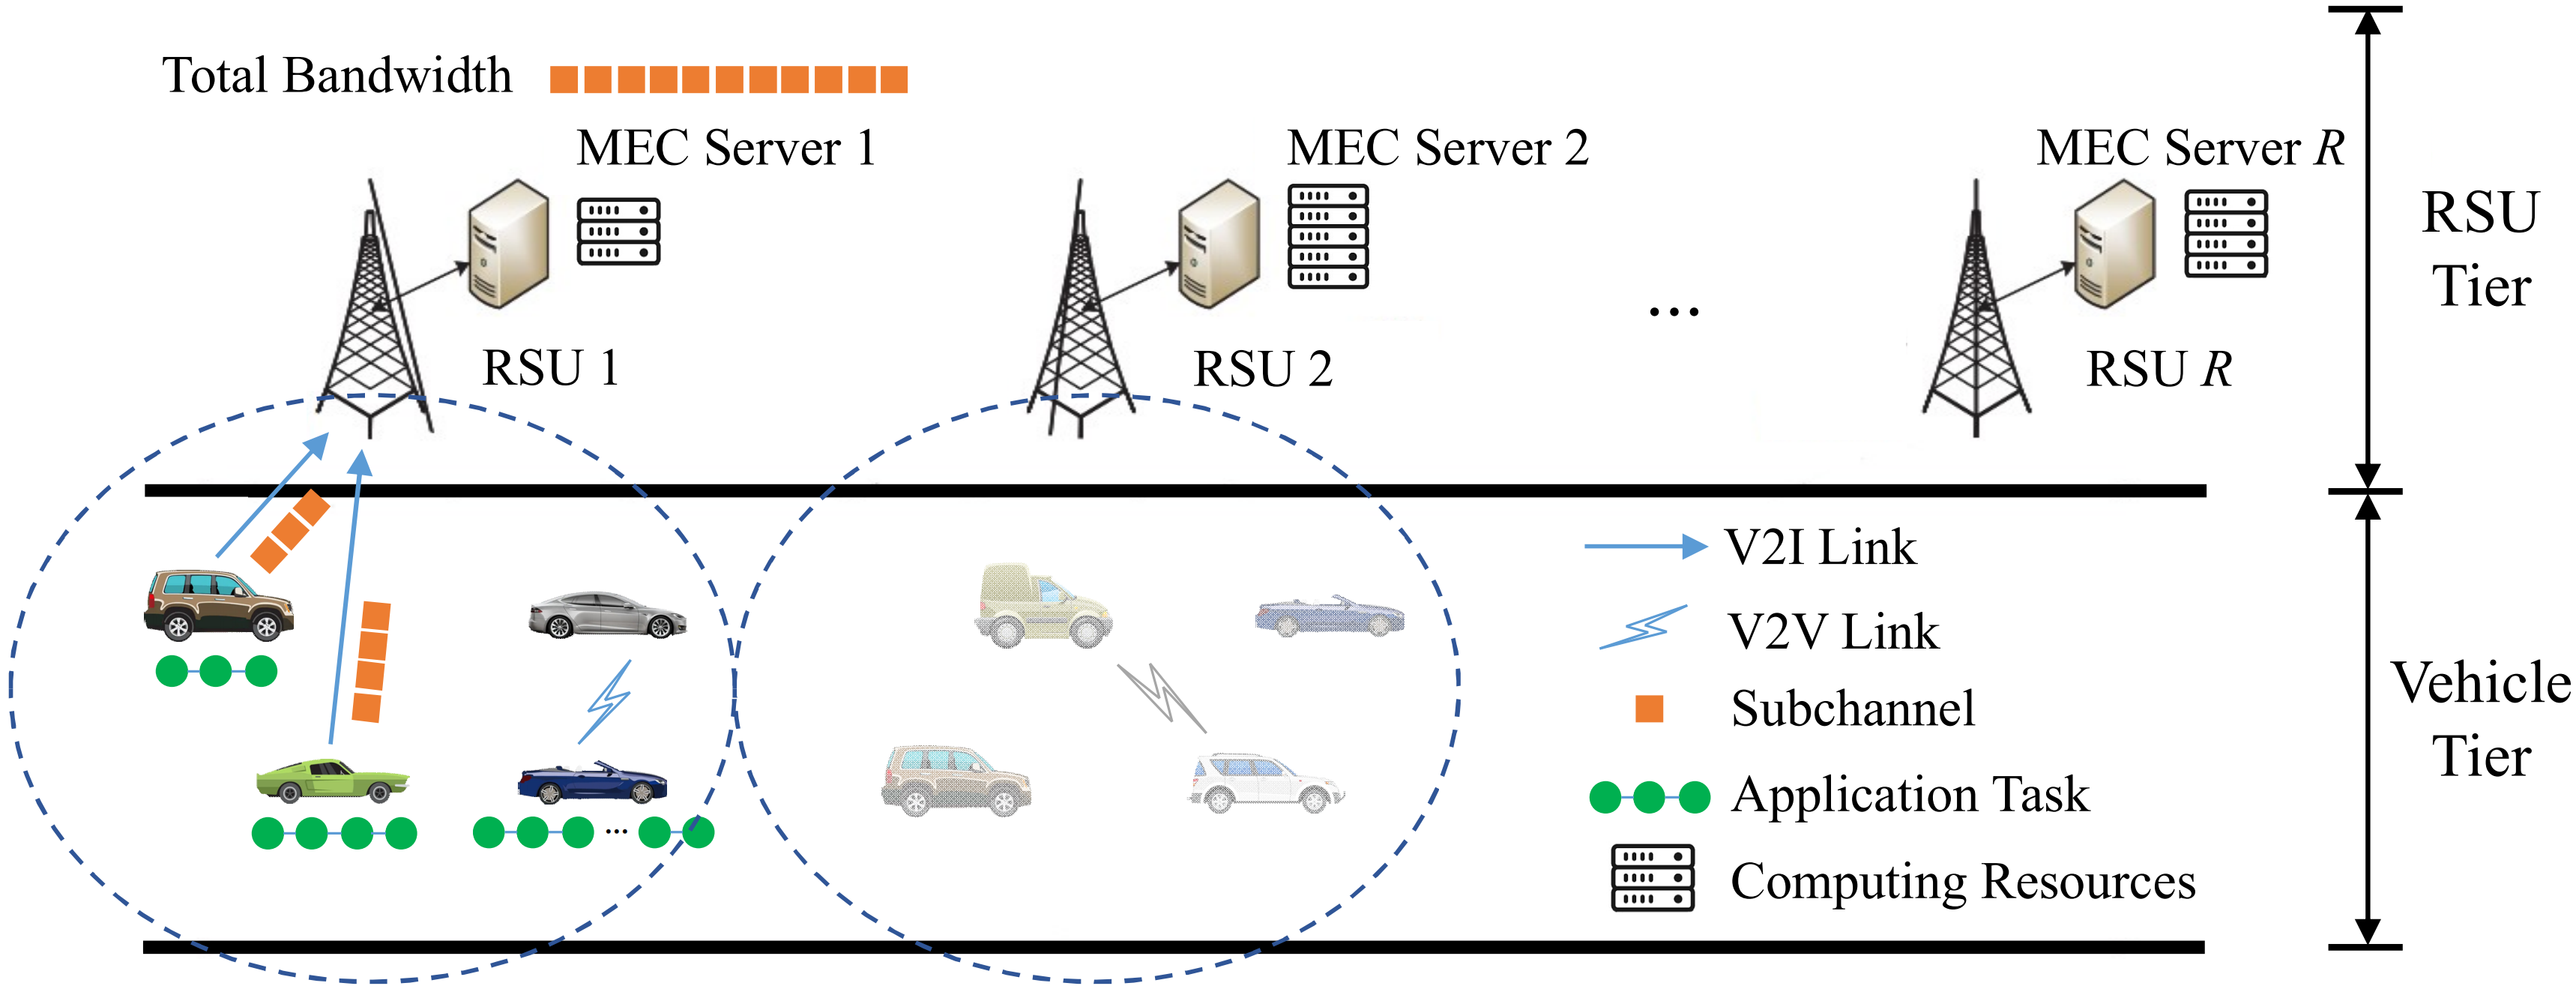
\includegraphics[width=3.5 in]{Figures/System_Model_TVT_R1.png}
\caption{The system model of the two-tier MEC-enabled vehicular network.}
\label{fig_1}
\end{figure}

% \IEEEpubidadjcol

The research system is illustrated in Fig. 1.  It consists of two tiers in the MEC-enabled vehicular network: the Vehicle Tier and the RSU Tier. RSUs can exchange data through wired communication and each is equipped with an MEC server that provides computing services for vehicles. They have different computing resources represented by varying numbers of chips. There are several vehicles in the service range of RSU$_1$ and each of them has an onboard computer with certain computing power. Some of the vehicles generate application tasks with sequential subtasks (as the the green circle strings show) to be executed. 


We define $\mathcal{N}=\{1,2, ..., n, ...,N\}$ as the set of needing vehicles (NVs) that are unable to complete their tasks on time and thus require external assistance. $\mathcal{IV}=\{1,2, ..., i, ...,I\}$ represents the set of idle vehicles (IVs) with idle computing resources that do not have tasks to be processed. Their computing capacities are highly variable. The vehicles capable of completing their tasks on time are not within the scope of this study. The set of RSUs is signified by $\mathcal{R}=\{1,2, ..., r, ...,R\}$. RSU and MEC server can be used interchangeably in this article, so we will use RSU uniformly in the remaining part. We employ the Cartesian coordinate system to describe the positions of devices, where the positive direction of $x$-axis aligns with the driving direction of vehicles, and the positive direction of $y$-axis is perpendicular to the road and upward. We denote the horizontal positions of NV$_n$, IV$_i$, and RSU$_r$ by $L_n = (x_n, y_n)$, $L_i = (x_i, y_i)$, and $L_r = (x_r, y_r)$, respectively. The height of RSU$_r$ is $H_r$. The velocities of NV$_n$ and IV$_i$ are signified as $v_n$ and $v_i$. The total system bandwidth $B$ of RSU$_1$ is divided into $b$ subchannels as the orange squares show. Each V2I (i.e., vehicle to RSU$_1$) uplink will be allocated a certain number of subchannels for data uploading.


We assume that each NV only has at most one application task to be computed and can only be associated with one RSU at a certain time, that is the RSU serving the current range. RSUs compute application tasks uni-directionally (i.e., following the vehicle driving direction) and no back-and-forth data transmission among RSUs. In this research, the applications we consider are object detection and recognition tasks in traffic environments, such as vehicle/pedestrian/obstacle detection and traffic sign recognition, etc. The results of such tasks are typically the coordinates of bounding box vertices or the categories of objects, which can be represented by a small amount of data. Therefore, similar to \cite{ref12},\cite{ref13}, we neglect the size of result data, and thus the process of transmitting it back to NV is not the focus of our research.

The task offloading process is described as follows. Firstly, we aim to match as many NVs as possible with a suitable IV as a helper in the Vehicle Tier to collaboratively compute their application tasks. The IVs that are ultimately selected to assist NVs will be referred to as the helping vehicles (HVs), denoted by set $\mathcal{H}=\{1,2, ..., h, ...,H\}$, and we have $\mathcal{H} \subseteq \mathcal{IV}$. These will be further elaborated in Tier-1, namely the Vehicle Tier. For the NVs that fail to be successfully matched in the Vehicle Tier, they will offload their application tasks to RSUs, which will then collaboratively compute tasks for NVs. These will be investigated in Tier-2, specifically the RSU Tier.


% \begin{figure}[h]
% \centering
% \includegraphics[width=2.6 in]{Figures_R4/Flow_Chart_R4.png}

% \captionsetup{justification = centering}
% \caption{Task offloading flow chart.}
% \label{fig_2}
% \end{figure}




\begin{table}[!t]
% \captionsetup{textfont=bf}
\caption{Main Notations and Definitions}
\label{tab:table1}
\centering
\begin{tabular}{|m{1.0cm}<{\centering}|m{1.0cm}<{\centering}|m{5.6cm}<{\centering}|}
\hline
Related Tier & Notations & Definitions\\
\hline
\multirow{8}{*}{General} & $C^n_m$ & Computation workloads of the $m\mbox{-}th$ subtask in the application task of NV$_n$\\
\cline{2-3} &
$W^n_{m-1,m}$ & Amount of intermediate data between subtask $m-1$ and $m$ in the application task of NV$_n$\\
\cline{2-3} &
$T_{n,max}$ & Latency requirement of the application task generated by NV$_n$\\
\cline{2-3} &
$W_0(x)$ & The principal branch of the Lambert W function \cite{ref28} and satisfies $W_0(x)e^{W_0(x)}=x$ and $W_0(x)\geq -1$\\
\hline
\multirow{13}{*}{Tier-1} & $B_{V2V}$ & Bandwidth for V2V communication\\
\cline{2-3} &
$C_{m_h}$ & The first subtask computed by HV$_h$\\
\cline{2-3} &
$\tau_{n,h}$ & V2V data transmission delay from NV$_n$ to HV$_h$\\
\cline{2-3} &
$E^{t}_{n,h}$ & V2V data transmission energy consumption from NV$_n$ to HV$_h$\\
\cline{2-3} &
$F_n$ & Maximal computing resources of NV$_n$\\
\cline{2-3} &
$F_h$ & Maximal computing resources of HV$_h$\\
\cline{2-3} &
$f^n_m$ & Computing resources allocated by NV$_n$ to its $m\mbox{-}th$ subtask\\
\cline{2-3} &
$f^h_m$ & Computing resources allocated by HV$_h$ to the $m\mbox{-}th$ subtask of NV$_n$\\
\cline{2-3} &
$\tau_{n,m}^c$ & Computation delay of the $m\mbox{-}th$ subtask of NV$_n$\\
\cline{2-3} &
$E_{n,m}^c$ & Computation energy consumption of the $m\mbox{-}th$ subtask of NV$_n$\\
\hline
\multirow{18}{*}{Tier-2} & $B$ & Total V2I bandwidth of RSU$_1$\\
\cline{2-3} &
$B_0$ & Bandwidth of each subchannel\\
\cline{2-3} &
$b_n$ & Number of subchannels allocated to the V2I link between NV$_n$ and RSU$_1$\\
\cline{2-3} &
$C^n_{m_r}$ & The first subtask of NV$_n$ computed by RSU$_r$\\
\cline{2-3} &
$\tau_{n}$ & Data transmission delay from NV$_n$ to RSU$_1$\\
\cline{2-3} &
$E^t_{n}$ & Data transmission energy consumption from NV$_n$ to RSU$_1$\\
\cline{2-3} &
$\tau_{r,n}$ & Data transmission delay of NV$_n$ from RSU$_r$ to RSU$_{r+1}$\\
\cline{2-3} &
$E^t_{r,n}$ & Data transmission energy consumption of NV$_n$ from RSU$_r$ to RSU$_{r+1}$\\
\cline{2-3} &
$F_r$ & Maximal computing resources of RSU$_r$\\
\cline{2-3} &
$f^r_{n,m}$ & Computing resources allocated by RSU$_r$ to the $m\mbox{-}th$ subtask of NV$_n$\\
\cline{2-3} &
$\tau^c_{n,m}$ & Computation delay of the $m\mbox{-}th$ subtask of NV$_n$\\
\cline{2-3} &
$E^{c}_{n,m}$ & Computation energy consumption of the $m\mbox{-}th$ subtask of NV$_n$\\
\hline

\end{tabular}
\end{table}


With the above establishment of the system, the application task, communication and computation models will be presented in the following. The main notations and the corresponding definitions in this research are summarized in TABLE I.


\subsection{Application Task Model}

\begin{figure}[h]
\centering
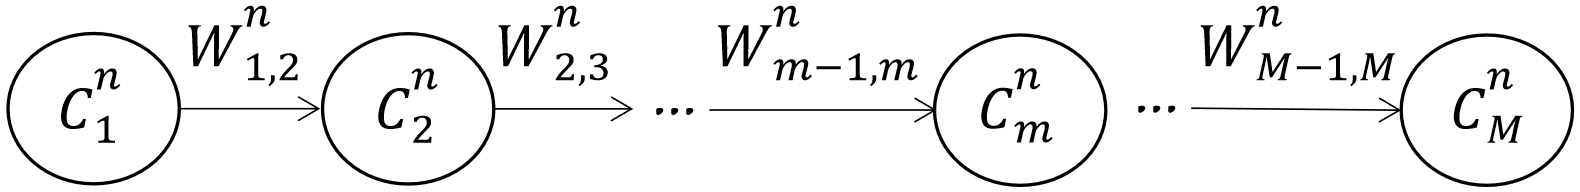
\includegraphics[width=3.3 in]{Figures/Task_Model_R4.png}
\caption{Application task model.}
\label{fig_2}
\end{figure}

We target at application tasks whose subtasks exhibit sequential dependencies. Only after the previous subtask is completed and its output data is obtained can the next subtask begin to be computed. Thus, we model the application task as a unidirectional graph as shown in Fig. 2. Each node represents a subtask, and each edge shows the dependency between adjacent subtasks.

We use set $\mathcal{M}^n=\{1,2, ...,M^n\}$ to denote the subtasks of the application task for NV$_n$, with the delay requirement signified by $T_{n,max}$. The computation workloads of the $m\mbox{-}th$ subtask of NV$_n$ is $C^n_m , m\in\mathcal{M}^n$, with the unit of CPU cycles. $W^n_{m-1,m}$ denotes the size of intermediate data between the $m-1\mbox{-}th$ and $m\mbox{-}th$ subtask in bits.



\subsection{Communication Model}

The subtask assignment of an application task on different devices is represented by the following notations. In the Vehicle Tier, for each NV$_n$, its subtasks $C_1^n , ..., C_{m_h-1}^n$ are computed locally on this NV, and subtasks $C_{m_h}^n , ..., C_M^n$ are computed on its matched HV$_h$. In the RSU Tier, each NV$_n$'s subtasks $C^n_{m_r} , ..., C^n_{m_{r+1}-1}$ are computed on RSU$_r$. The last RSU$_R$ computes subtask $C^n_{m_R} , ..., C^n_M$.

Based on the above establishment, for the Vehicle Tier, NV$_n$ offloads subtasks starting from $C_{m_h}^n$. Therefore, NV$_n$ will transmit the input data of the $m_h\mbox{-}th$ subtask (i.e., with the data size of $W_{m_h-1,m_h}^n$) to its matched HV$_h$. Similar to \cite{ref16,ref21}, we adopt Orthogonal Frequency Division Multiplexing (OFDM) and Orthogonal Frequency Division Multiple Access (OFDMA) technologies for V2V and V2I communications, respectively. Each communication link occupies mutually orthogonal subbands, which exhibits strong resistance to signal interference. Assuming the bandwidth for V2V communication is $B_{V2V}$, the V2V transmission delay from NV$_n$ to HV$_h$ is denoted by $\tau_{n,h}$, the transmission energy consumption is $E^t_{n,h}$ and the power spectrum density of noise at HV is $N_0$. Therefore, based on Shannon capacity formula, we can obtain\\
\begin{equation*}
W_{m_h-1,m_h}^n = \tau_{n,h}B_{V2V}\ln\left(1+\dfrac{E_{n,h}^t 10^{-\frac{\phi_{n,h}}{10}} h_{n,h}}{\tau_{n,h}B_{V2V}N_0}\right), \tag{1}
\end{equation*}
where $\phi_{n,h}=63.3+17.7\lg(d_{n,h})$ \cite{ref15} is the path loss between NV$_n$ and HV$_h$. $d_{n,h}$ denotes the Euclidean distance between them, which can be calculated based on their respective positions. $h_{n,h}$ is the channel fading factor between them.

Regarding the RSU Tier, since all the subtasks will be computed collaboratively by RSUs, the NV$_n$ needs to transmit the initial task data (i.e., the input data of the first subtask), with the data size $W^n_0$, to RSU$_1$. Assume that the total bandwidth of RSU$_1$ is $B$ and the bandwidth allocated to each V2I uplink from NV$_n$ to RSU$_1$ is $b_nB_0$, where $B_0$ is the bandwidth of each subchannel and $b_n$ signifies the number of subchannels allocated to each V2I uplink. We denote the V2I transmission delay of NV$_n$ as $\tau_{n}$, the transmission energy consumption as $E^t_{n}$ and the power spectrum density of noise at RSU$_1$ as $N_0$. Then we have\\
\begin{equation*}
W^n_0=\tau_{n}b_nB_0\ln\left(1+\dfrac{E_n^t \phi_n h_n}{\tau_{n}b_nB_0N_0}\right), \tag{2}
\end{equation*}
where $\phi_n = d_{n}^{-\delta}$ \cite{ref21} is defined as the path loss between NV$_n$ and RSU$_1$, with $d_{n}$ and $\delta$ denoting the distance between them and path loss factor, respectively.

Based on (1) and (2), the expression of V2V and V2I transmission energy consumption $E_{n,h}^t$ and $E_n^t$ can be rewritten as follows respectively\\
\begin{equation*}
E_{n,h}^t=\frac{B_{V2V}N_0\tau_{n,h}}{10^{-\frac{\phi_{n,h}}{10}} h_{n,h}}\left(e^{\frac{W_{m_h-1,m_h}^n}{\tau_{n,h}B_{V2V}}}-1\right), \tag{3}
\end{equation*}
\begin{equation*}
E^t_n=\dfrac{b_nB_0N_0\tau_{n}}{\phi_n h_n}\left(e^{\frac{W^n_0}{\tau_{n}b_nB_0}}-1\right). \tag{4}
\end{equation*}

We model the wired transmission among RSUs as follows. Suppose that the required energy for each RSU to transmit one bit of data to the next RSU through wired link is $E_0$ and the delay for transmitting one bit is $\tau_0$. Then the energy consumption for RSU$_r$ to transmit the intermediate data of NV$_n$ to RSU$_{r+1}$ can be expressed by $E^t_{r,n}=E_0W^n_{m_{r+1}-1,m_{r+1}}$ and the corresponding data transmission delay is $\tau_{r,n}=\tau_0W^n_{m_{r+1}-1,m_{r+1}}$.


\subsection{Computation Model}

We adopt a general CPU computation model so that the strategy in this paper is also applicable to other more specific scenarios. The CPU frequency $f$ (also known as CPU clock speed) is defined as the number of CPU cycles that can be processed per second. For a specific $f$, the computing power can be expressed by $\kappa f^3$, where $\kappa$ is the energy efficiency coefficient of the chip, a constant related to hardware \cite{ref8}. When the processor computes a task with the workloads of $C$ CPU cycles, the computation delay is $C/f$. Hence the computation energy consumption is $\kappa Cf^2$. We denote the $\kappa$ of NV$_n$, HV$_h$, and RSU$_r$ as $\kappa_n$, $\kappa_h$, and $\kappa_r$, respectively. The maximal CPU frequency (i.e., maximal computing resources) of NV$_n$, IV$_i$, HV$_h$, and RSU$_r$ are $F_n$, $F_i$, $F_h$, and $F_r$, respectively. In order to save energy, the working frequency of each device will be optimized instead of directly using the maximum.

In the Vehicle Tier, the CPU frequency allocated by each pair of NV$_n$ and HV$_h$ when computing the subtask $C_m^n$ are denoted by $f^n_m$ and $f^h_m$, respectively. According to the subtask assignment representation in Section II-C, the computation delay of each subtask, symbolized by $\tau_{n,m}^c$, can be expressed as $\tau_{n,m}^c=\frac{C_m^n}{f^n_m}, 1\leq m \leq m_h-1$ and $\tau_{n,m}^c=\frac{C_m^n}{f^h_m}, m_h\leq m \leq M^n$. The energy consumption for computing each subtask can be written as $E_{n,m}^c=\kappa_n C_m^n\left(f^n_m\right)^2, 1\leq m \leq m_h-1$ and $E_{n,m}^c=\kappa_h C_m^n\left(f^h_m\right)^2, m_h\leq m \leq M^n$. In the RSU Tier, we denote the CPU frequency allocated by RSU$_r$ to compute the subtask $C^n_m$ of NV$_n$ as $f^r_{n,m}$. Similarly, the computation delay and energy consumption of each subtask of NV$_n$ are $\tau^c_{n,m}=\frac{C_m^n}{f^r_{n,m}}$ and $E^{c}_{n,m}=\kappa_r C_m^n\left(f^r_{n,m}\right)^2, \forall n \in \mathcal{N}, m_r\leq m \leq m_{r+1}-1, \forall r \in \mathcal{R}$, respectively.


%%%%%%%%%%%%%%%%%%%%%%%%%%%%%%%%%%%%%%%%%%%%%%%%%%%%%%%%%%%%%%%%%%%%%%%%%%%%%%%%%%%%


\section{Tier-1: Collaborative Computation Between NV and HV in the Vehicle Tier}
In this section, we elaborate the study of the Vehicle Tier. We first present the NV-HV matching algorithm, followed by the formulation of the subproblem that minimizes vehicle energy consumption under the constraints of task delay requirements and computing resources of vehicles. Subsequently, we discuss the solution to this subproblem.


\subsection{NV-HV Matching}

Consider the scenario where initial system consists of $N$ NV and $I$ IV. After the matching process, the IV that are ultimately selected to serve as helpers for NV will become HV. In this subsection, we introduce the proposed NV-HV matching algorithm, which aims to match as many NV as possible with qualified HV in the Vehicle Tier.

We consider the positions and velocities of NVs and IVs, the computational workloads and delay requirements of each NV's task, as well as the maximum computing resources available for each IV similar to \cite{ref29}. The maximum V2V communication range is denoted by $D_{V2V}$. The matching algorithm consists of the following two parts:

(1) \textbf{Candidate NV-IV Matching Identification:} Only the NV-IV pair that simultaneously satisfies the following two conditions can be considered as a candidate match:
\begin{itemize} 

\item \textit{V2V Communication Range Condition}: The real-time distance between the two vehicles is less than $D_{V2V}$ or the distance is equal to $D_{V2V}$, but the vehicle positioned behind is driving at a higher speed than the one in front, implying that the two vehicles are approaching each other. Note that, to prevent communication interruption, the extreme case where the distance is equal to $D_{V2V}$ while the speeds of the two vehicles are identical is considered not to meet this condition.

\item \textit{IV Computing Resource Condition}: When the IV utilizes its maximum computing resources to process the NV's task, the corresponding computation delay must be shorter than the delay requirement of this task.

\end{itemize}
Through this process, we obtain all potential NV-IV matches. Note that by this point, each NV may have one, multiple, or no candidate IV.

(2) \textbf{Maximum Matching for NVs:} We resort to the Hungarian algorithm \cite{ref30} to perform the maximum matching for NVs based on the current set of candidate NV-IV matches. The selected IVs in the final matching are promoted to HVs. In this manner, we maximize the number of NV that can find suitable HV under the given system conditions in the Vehicle Tier. Subsequently, we further optimize the task offloading decision and the allocation strategies for communication and computation resources of each NV-HV pair.



\subsection{Problem Formulation of Vehicle Tier}
Afetr the determination of NV-HV pairs, in this subsection, we formulate the subproblem to jointly optimize task offloading decision, V2V transmission delay and computation resource allocation. The objective is to minimize the weighted sum energy consumption of vehicles while ensuring the delay requirements of NVs' application tasks can be met. The optimization problem $\mathcal{P}_1$ of Tier-1 is formulated as follows.

$\mathcal{P}_1:$ Collaborative computation of vehicles

\vspace{-0.5cm}
% \begin{small}
\begin{align*}
%\mathcal{P}_1:\\
\min _{\substack {\mathbf{m_h}, \mathbf{\tau_{n,h}},\\ \mathbf{f_m^V}}} &\sum_{h=1}^{H} \left[w_n \left ( E_{n,h}^t + \sum _{m=1}^{m_h-1} E_{n,m}^c \right) + w_h \sum_{m=m_h}^{M^n} E_{n,m}^c \right]\\
\text {s.t. } \hspace{0.1cm} &1 \leq m_h \leq M^n, \forall h \in \mathcal {H}, \tag{5a}\\
& \sum_{m=1}^{M^n} \tau_{n,m}^c +\tau_{n,h} \leq T_{n,max}, \forall h \in \mathcal {H}, \tag{5b}\\
& \tau_{n,h} \geq 0, \forall h \in \mathcal {H}, \tag{5c}\\
& 0 \leq f^n_m \leq F_n, m=1,...,m_h-1, \forall h \in \mathcal {H},\tag{5d}\\
& 0 \leq f^h_m \leq F_h, m=m_h,...,M^n, \forall h \in \mathcal {H}. \tag{5e}
\end{align*}
% \end{small}


In the objective function, the first two terms are the V2V data transmission energy and the computation energy of the first $m_h-1$ subtasks consumed by each NV, respectively. HV's energy consumption for computing the remaining subtasks is represented by the last term. The $w_n$ and $w_h$ are the weights of NV$_n$ and HV$_h$, respectively. Note that not all NVs can be matched in the Vehicle Tier. Therefore, we use the index $n$ of HV to correspond to each NV-HV pair.

Regarding the optimization variables, set $\mathbf{m_h}=\{m_h|h \in \mathcal{H}\}$ encompasses the index of the first subtask computed on each HV, indicating the offloading decision for each pair. The V2V data transmission delays are denoted by $\mathbf{\tau_{n,h}}=\{\tau_{n,h}| h \in \mathcal{H}\}$. Set $\mathbf{f_m^V}$ is the union of $\left\{ f^n_m|m=1,...,m_h-1 \right\} $ and $ \left\{f^h_m|m=m_h,...,M^n \right\}$, $\forall h \in \mathcal{H}$, including the computing resources allocated by the two types of vehicles to compute each subtask.

In terms of the constraints, (5a) limits the range of each $m_h$. The total execution delay does not exceed the required delay of each application is guaranteed by (5b). Constraint (5c) ensures the nonnegativity of the transmission delay. The allocated computing resources by the two types of vehicles to each subtask will not be greater than their maximal computing resources are guaranteed by (5d) and (5e).


\subsection{Problem Solving}
To solve this MINLP problem, our strategy is to decompose $\mathcal{P}_1$ into two subproblems. In the first subproblem $\mathcal{P}_{1-1}$, we initially fix the integer variable $m_h$ and then optimize the remaining two types of continuous variables. In the second subproblem $\mathcal{P}_{1-2}$, the optimal $m_h^*$ for each NV-HV pair is determined via the exhaustive searching.

For the convenience of presentation, we make the following definitions for each pair:
\begin{align*}
f^{V}_{m} \triangleq \begin{cases} f^n_m, & m=1,\ldots, m_h-1, \\ f^h_m, & m=m_h,\ldots, M^n, \end{cases}\tag{6}\end{align*}

\begin{align*}
F_V \triangleq \begin{cases} F_n, & m=1,\ldots, m_h-1, \\ F_h, & m=m_h,\ldots, M^n. \end{cases}\tag{7}\end{align*} 
Through the above definitions, we combine equations (5d) and (5e) into
\begin{align*}
0 \leq f^{V}_{m} \leq F_V, m=1,...,M^n. \tag{8}
\end{align*}


\textbf{Proposition 1:} \textit{$\mathcal{P}_{1-1}$ is a convex optimization problem.}

\emph{Proof:} Regarding the objective function, the second-order derivative of the first term $w_nE_{n,h}^t$ with respect to $\tau_{n,h}$ is always greater than zero, indicating the convexity with respect to $\tau_{n,h}$. The second and third terms are convex functions with respect to $f^n_m$ and $f^h_m$, respectively. Since the objective function is the summation of such convex functions, it is also convex. As for the constraints, the function $\frac{C_m^n}{f^{V}_{m}}$ in the first term of constraint (5b) is convex with $f^{V}_{m}$ and constraint (8) are affine functions of $f^{V}_{m}$ that are also convex. Additionally, the constraints (5b) and (5c) are all affine and convex with $\tau_{n,h}$. This completes the proof.
$\hfill\blacksquare$

The convexity of this problem indicates that we can directly derive globally optimal solution that meets the delay requirements while minimizing vehicle energy consumption. Coupled with the satisfaction of Slater's condition, it can be efficiently solved by the Karush-Kuhn-Tucker (KKT) conditions algorithm with low complexity. The fast execution speed of algorithm is well suited for real-time decision-making demand in highly dynamic traffic environment. Then we can derive the optimal solutions of $\tau_{n,h}$ and $f^{V}_{m}$ as presented in the following.

\emph{Lemma 1:} The optimal V2V transmission delay for each NV-HV pair is:
% {\setlength\abovedisplayskip{4pt}
% \setlength\belowdisplayskip{4pt}
% \vspace{-0.7cm}
\begin{equation*}
\tau^*_{n,h}=\frac {W_{m_h-1,m_h}^n}{B_{V2V} \left [{W_{0} \left ({\frac {\frac{10^{-\frac{\phi_{n,h}}{10}} h_{n,h}\lambda }{w_n N_0B_{V2V}}-1}{e}}\right)+1 }\right]}. \tag{9}
\end{equation*}


\emph{Proof:} The KKT conditions formulas of the problem $\mathcal{P}_{1-1}$ are listed as following:
\vspace{-0.2cm}
\begin{align*}
&\text{Constraints (5b), (5c) and (8),}  \\
&\lambda \left( \sum_{m=1}^{M^n} \frac{C_m^n}{f^{V}_{m}}+\tau_{n,h} - T_{n,max}\right) = 0, \tag{10a}\\
&\eta \tau_{n,h} = 0, \tag{10b}\\
&\mu_m f^V_{m} = 0, m=1,\ldots,M^n, \tag{10c}\\
&\nu_m \left(f^V_{m}-F_V\right) = 0, m=1,\ldots,M^n, \tag{10d}\\
&\frac {w_nB_{V2V}N_0}{10^{-\frac{\phi_{n,h}}{10}} h_{n,h}} \left( e^{\frac {W_{m_h-1,m_h}^n}{\tau _{n,h}B_{V2V}}}-1\right) \\
&-\frac {w_n N_0 W_{m_h-1,m_h}^n e^{\frac {W_{m_h-1,m_h}^n }{\tau _{n,h}B_{V2V}}}}{10^{-\frac{\phi_{n,h}}{10}} h_{n,h}\tau _{n,h}} +\lambda -\eta =0, \hspace{0.9cm} \tag{10e}\\
&2w_n\kappa_{n} C_m^n f^{V}_{m} -\lambda \frac{C_m^n}{\left ({f^{V}_{m}}\right)^{2}} -\mu _{m} + \nu _{m}=0,\\
&m=1,\ldots, m_h-1, \tag{10f}\\
&2w_h\kappa_{h} C_m^n f^{V}_{m} -\lambda \frac{C_m^n}{\left ({f^{V}_{m}}\right)^{2}} -\mu _{m} + \nu _{m}=0,\\
&m=m_h,\ldots, M^n. \tag{10g}\\
\end{align*}
where $\lambda$, $\eta$, $\mu_m$ and $\nu_m$ are the nonnegative Lagrange multipliers associated with the constraint (5b), (5c), $f^V_{m}\geq 0$ and $f^V_{m}\leq F_V$, respectively.

We have $\tau_{n,h}>0$ to guarantee the rationality. Therefore, we have $\eta=0$ based on (10b). We can define $d\triangleq\frac{W_{m_h-1,m_h}^n}{B_{V2V}\tau_{n,h}}$. Therefore, the formula (10e) can be expressed as
\begin{equation*}
(d-1)e^{d-1}=\frac{\frac{10^{-\frac{\phi_{n,h}}{10}} h_{n,h}\lambda}{w_n N_0 B_{V2V}}-1}{e}. \tag{11}
\end{equation*}

In order to obtain the optimal expression of $\tau_{n,h}$, we leverage the function $W_0(x)$ whose definition is given in TABLE I. Since $d>0$, we have $d-1 > -1$. Therefore, we can obtain
\begin{equation*}
d=W_0\left(\frac{\frac{10^{-\frac{\phi_{n,h}}{10}} h_{n,h}\lambda}{w_n N_0 B_{V2V}}-1}{e}\right)+1. \tag{12}
\end{equation*}
Then we substitute the defined expression of $d$ into (12) and we can finally get the optimal solution as given in (9).$\hfill\blacksquare$


\emph{Lemma 2:} The optimal allocation of computing resource for each subtask by NV and HV is:
\begin{equation*}
{f^V_{m}}^*=\min \left ({\left ({\frac {\lambda }{2w_{g(m)}\kappa _{g(m)}}}\right)^{\frac {1}{3}}, F_V}\right), m=1,\ldots, M^n, \tag{13}
\end{equation*}
where $g(m)$ is $n$\footnote{The $n$ and $h$ here are only two indices representing NV$_n$ and HV$_h$, respectively.} when $1 \leq m \leq m_h-1$ and $h$ when $m_h \leq m \leq M^n$. The optimal value of $\lambda$ can be easily found using the bisection searching method.


\emph{Proof:} According to the function $\frac{C_m^n}{f^V_{m}}$ in the first term of (5b), we should restrict $f^V_{m}\neq0$, and we have $\mu_m=0$ based on (10c). We focus on the solution of $\left\{f^{V}_{m}|m=1,\ldots,m_h-1 \right\}$ and optimal $\left\{f^{V}_{m}|m=m_h,\ldots,M^n \right\}$ can be obtained similarly.

For $m=1,\ldots,m_h-1$, when $0<f^{V}_{m}<F_V$, then $\nu_m = 0$ according to (10d). Thus, we can rewrite the (10f) as
{\setlength\abovedisplayskip{8pt}
\setlength\belowdisplayskip{8pt}
\begin{equation*}
2w_n\kappa_n C_m^n f^{V}_{m}=\lambda \frac {C_m^n}{\left ({f^V_{m}}\right)^{2}}. \tag{14}
\end{equation*}}
The computing resources allocated to each subtask becomes
{\setlength\abovedisplayskip{8pt}
\setlength\belowdisplayskip{8pt}
\begin{equation*}
f^V_{m}=\left(\frac{\lambda}{2w_n\kappa_n}\right)^{\frac{1}{3}}. \tag{15}
\end{equation*}}
When $f^{V}_{m}=F_V$, then $\nu_m\geq0$. Hence (10f) can be rewritten as
{\setlength\abovedisplayskip{8pt}
\setlength\belowdisplayskip{8pt}
\begin{equation*}
2w_n\kappa_n C_m^n f^{V}_{m}+\nu_m=\lambda \frac {C_m^n}{\left ({f^V_{m}}\right)^{2}}, \tag{16}
\end{equation*}}
where $f^V_{m}$ can be replaced by $F_V$. Assuming that for
$m \in \left\{1,\ldots,m_h-1\right\}$, some of them have the expression of $f^V_{m}$ satisfying (15) while some have $f^{V}_{m}=F_V$. This means that equations (14) and (16) hold simultaneously. We can obtain the following inequality chain
\begin{align*}
\lambda &\overset{\text{(a)}}{=} 2w_n\kappa_n \left(F_V\right)^3 + \nu_m \frac{\left(F_V\right)^2}{C_m^n} \\
&\overset{\text{(b)}}{\geq} 2w_n\kappa_n \left(F_V\right)^3 \\
&\overset{\text{(c)}}{>} 2w_n\kappa_n \left(f^V_{m}\right)^3 \\
&\overset{\text{(d)}}{=} \lambda. \tag{17}\\
\end{align*}
(a) is transformed from (16) and the inequality (b) holds due to $\nu_m\geq0$. When $0<f^{V}_{m}<F_V$, we have (c), which is also the expression of $\lambda$. We can find that there is a contradiction. Thus, for the $m \in \left\{1,\ldots,m_h-1\right\}$, all the $f^V_{m}$ will follow one of these two formulas, i.e., (15) or $f^{V}_{m}=F_V$.

Then we present under what circumstances which one should be followed. Obviously, the upper bound for the value of $\lambda$ is $2w_n\kappa_n\left(F_V\right)^3$. Suppose that when $\lambda < 2w_n\kappa_n\left(F_V\right)^3$, the $f^{V}_{m}=F_V, m=1,\ldots,m_h-1$ is followed. In this case, $\nu_m\geq0$ and still $\mu_m=0$. According to (10f), we have
\begin{align*}
\lambda &= 2w_n\kappa_n \left(F_V\right)^3 + \nu_m \frac{\left(F_V\right)^2}{C_m^n}\\
&\geq 2w_n\kappa_n \left(F_V\right)^3. \tag{18}\\
\end{align*}
There is a contradiction. Therefore, when $\lambda < 2w_n\kappa_n\left(F_V\right)^3$, the optimal solution of $f^V_{m}$ should be (15). When $\lambda \geq 2w_n\kappa_n\left(F_V\right)^3$, if (15) is followed, we have $f^V_{m} \geq F_V$. This violates the constraint (8). Thus, the optimal solution is $f^{V}_{m}=F_V$ in this case. We merge the optimal expressions of $\left\{f^{V}_{m}|m=1,\ldots,M^n \right\}$ into (13).

By this point, we express the optimal transmission delay and computing resource allocation policy as the functions of $\lambda$. Then the condition that the $\lambda^*$ satisfies and the method for obtaining it are given as follows. In the objective function of $\mathcal{P}_{1-1}$, the first term is monotonically decreasing with $\tau_{n,h}$ when $\tau_{n,h}>0$ (this can be easily proved by second-order derivative) and the rest two terms are monotonically increasing with $f^n_m$ and $f^h_m$, respectively. Based on (9), $\tau_{n,h}^*$ is monotonically decreasing with $\lambda$, while (13) indicating that ${f^V_{m}}^*$ are monotonically nondecreasing with $\lambda$. Therefore, the objective function is monotonically increasing with $\lambda$. To minimize the function value, $\lambda$ should be as small as possible.

As for the constraint (5b), the function in the left-hand side is monotonically decreasing with $\lambda$. Thus, we only need to find the $\lambda$ that activates the inequality (5b). Due to the monotonicity, this value can be found using the bisection searching method. $\hfill\blacksquare$

\subsection{Complexity Analysis}
The complexity of the NV-HV matching algorithm consists of two parts: candidate NV-IV matching identification and maximum matching for NVs. The first part needs to iterate through all NV-IV pairs to verify whether they meet V2V communication range and IV computing resource conditions. Consequently, the complexity of this part is $\mathcal{O}\left( N I \right)$. The method for maximum matching is to search for augmenting paths. For each NV, in the worst case, it may need to traverse all edges (i.e., the candidate matches in the adjacency list obtained from the first part). Hence, the complexity of the second part is $\mathcal{O}\left( N^2I \right)$. The overall worst-case complexity of the matching algorithm is $\mathcal{O}\left( NI+N^2I \right) 
\approx \mathcal{O}\left( N^2I \right)$. When the adjacency list is sparse, the complexity will be significantly reduced. Obtaining the optimal task offloading decision for each matched NV requires traversing its subtasks, resulting in a complexity of $\mathcal{O}\left( H \overline{M} \right)$, where $\overline{M}$ represents the average number of subtasks for each application. Note that the reason for using the number of HVs $H$ here is that it is equivalent to the number of NVs successfully matched in the Vehicle Tier. The optimal V2V transmission delay and computing resource allocation strategy can be directly derived by substituting the known parameters into the optimal solution expressions, which belong to constant time complexity. Consequently, the overall complexity of the method in the Vehicle Tier is $\mathcal{O}\left( N^2 I + H \overline{M} \right)$.


%%%%%%%%%%%%%%%%%%%%%%%%%%%%%%%%%%%%%%%%%%%%%%%%%%%%%%%%%%%%%%%%%%%%%%%%%%%%%%%%%%%%


\section{Tier-2: Collaborative Computation in the RSU Tier}

In this section, the cooperation among RSUs to compute the application tasks for NVs is investigated. The NVs that fail to be successfully matched with a suitable HV in the Vehicle Tier will offload their tasks to RSU. After that, each RSU will compute several subtasks and transmit the intermediate data to the next RSU for further computation.


\subsection{Problem Formulation of RSU Tier}
Compared with Tier-1, each RSU will serve multiple NVs, and thus we further address the multi-access issues for bandwidth and computing resource allocation. In this tier, the NVs being served are those that failed to be matched in the Vehicle Tier, symbolized by the set $\mathcal{N}'$ with a total number of $N'$. We formulate the optimization problem $\mathcal{P}_2$ of the RSU Tier as shown at the bottom of the next page.

\begin{figure*}[!b]
\centering
% \hline
\rule{52em}{0.5pt}
\begin{align*}
\mathcal{P}_2: \text{Collaborative computation of RSUs}\\
\min _{\substack { \mathbf{m^n_r} , \mathbf{\tau_n},   \mathbf{f^{r}_{n,m^n}}, \mathbf{b_n}}} \hspace{0.3cm} &\sum^{N'}_{n=1} \left[ w_n E^t_{n} + \sum_{r=1}^{R} w_r \left( E^t_{r,n} + \sum_{m^n=m_r^n}^{m_{r+1}^n-1} E^{c}_{n,m} \right) \right]\\
\text {s.t. } \hspace{0.9cm} & 1 \leq m_1^n \leq \cdots \leq m_r^n \leq m_{r+1}^n \leq \cdots \leq M^n +1, n \in \mathcal {N'}, r \in \mathcal{R}, \hspace{0.5cm} \tag{19a}\\
& \sum_{q=1}^{Q^n} \frac{D^n_q}{R_{n}} + \tau_{n}+\sum_{r=1}^{R}\sum_{m^n=m^n_r}^{m^n_{r+1}-1}\tau^{c}_{n,m} + \sum_{r=1}^{R-1}\tau_{r,n} \leq T_{n,max}, n \in \mathcal{N'}, \tag{19b}\\
& \sum_{q=1}^{Q^n} \frac{D^n_q}{R_{n}} + \tau_{n} \leq \frac{L-S_n}{v_n}, n \in \mathcal{N'}, \tag{19c}\\
& 0 \leq \tau_{n} \leq \tau_{max}, n \in \mathcal{N'}, \tag{19d}\\
& \sum_{n=1}^{N'} b_n \leq b, b_n \in \mathcal{I}_+, \tag{19e}\\
& 0 \leq \sum_{n=1}^{N'} f^{r}_{n,m^n} \leq F_r, r \in \mathcal{R}. \tag{19f}
\end{align*}
\end{figure*}


The objective function consists of the energy consumption of data transmission from NVs to RSU$_1$, data transmission from each RSU$_r$ to the next RSU, and computation on RSUs, respectively. Note that the second term of the RSU that computes the last subtask of NV$_n$ is zero since it does not need to transmit data. $w_n$ and $w_r$ are the weights of NV$_n$ and RSU$_r$. Then the objective function is the summation of the energy consumption for each NV$_n$.

The optimization variables are categorized into four sets. The first set $\mathbf{m_r^n} = \left\{ m^n_r|n \in \mathcal{N}, r \in \mathcal{R} \right\}$ consists of the task offloading decisions for all NVs' application tasks. The second set $\mathbf{\tau_n} = \left\{ \tau_{n}|n \in \mathcal{N} \right\}$ comprises the data transmission delays from each NV$_n$ to RSU$_1$. The third set $\mathbf{f^{r}_{n,m^n}} = \left\{ f^{r}_{n,m^n}|m^n \in \mathcal{M}^n,n \in \mathcal{N},r \in \mathcal{R} \right\}$ contains the computing resource allocation policy for each subtask of each NV. Lastly, the fourth set $\mathbf{b_n} = \left \{b_n|n \in \mathcal {N}\right \}$ includes the number of subchannels allocated to each V2I link.

As for the constraints, (19a) ensures the relationship and the range of task offloading decisions (i.e., $m^n_r$) for each NV$_n$. In (19b), the first term is the communication setup delay between each NV$_n$ and RSU$_1$, where $Q^n$ signifies the total number of the communication setup messages of NV$_n$, $D^n_q$ denotes the data size of the $q\mbox{-}th$ setup message of NV$_n$, and $R_{n}$ is the data rate of the communication link dedicated for the transmission of the NV$_n$'s setup messages. The following two terms are the V2I data transmission delay and the sum of computation delay on RSUs, respectively. The data transmission delays from an RSU to the next one are summed in the last term. Hence (19b) guarantees the total execution delay of the NV$_n$'s application task will not exceed its delay requirement. (19c) is related to the mobility of NVs, where $L$ is the length of RSU$_1$'s service range, $S_n$ denotes the distance from the starting point of service range to the current position of NV$_n$. Thus, it guarantees that NV$_n$ completes communication setup and data uploading with RSU$_1$ before leaving its service range. (19d) ensures the data transmission delays are nonnegative and not greater than a tolerant threshold $\tau_{max}$. The sum of subchannels allocated to each V2I link should not exceed the total available number of subchannels $b$ is guaranteed by (19e), where $\mathcal{I}_+$ is the set of positive integers. (19f) ensures the summation of the allocated computation resources should not exceed the available resources of the corresponding RSU.


\emph{Remark:} In constraint (19a), $m^n_r=m^n_{r+1}$ means the RSU$_r$ is not assigned any subtask of NV$_n$ and only needs to transmit data to RSU$_{r+1}$. These RSUs are referred to as TYPE 1 RSUs. When $m^n_r=M^n+1$, it means previous RSUs have completed all the subtasks of NV$_n$. Hence the RSU$_r$ will do nothing for NV$_n$. We call them TYPE 2 RSUs. Therefore, in the objective function and the constraint (19b), the computation delay and energy consumption of TYPE 1 RSUs are zero, while all the delay and energy consumption for both of transmission and computation of TYPE 2 RSUs are zero.
% \vspace{-0.2cm}

\subsection{Solutions to Allocation Policies of Communication and Computation Resources}
Similar to $\mathcal{P}_1$, we decompose the problem $\mathcal{P}_2$ into two subproblems. In subproblem $\mathcal{P}_{2-1}$, we begin by fixing the integer variable set $\mathbf{m_r^n}$ and then optimize the remaining variables. Subsequently, the optimal values of each $m^n_r$ can be obtained in the second subproblem $\mathcal{P}_{2-2}$. This subsection presents the solving process for continuous variables.

For notational simplicity, we make the following definition:
\begin{align*}
f_{n,m^n} \triangleq f^{r}_{n,m^n}, m^n=m^n_r,\ldots, m^n_{r+1}-1. \tag{20}\end{align*}
For the RSU that computes the last subtask of NV$_n$, $m^n_{r+1}-1=M^n$. Based on the above definition, we can rewrite the third term in (19b) by merging the computation delay of each RSU to compute subtasks for NV$_n$ into $\sum_{m^n=1}^{M^n}\frac{C^n_m}{f_{n,m^n}}$. We have another definition as
\begin{align*}
F \triangleq F_r, m^n= m^n_r, \ldots, m^n_{r+1}-1.\tag{21}\end{align*} 
According to the above definition, (19f) can be transformed into the following constraint:
\begin{align*}
0 \leq \sum_{n=1}^{N'} f_{n,m^n} \leq F, m^n \in \mathcal{M}^n. \tag{22}\end{align*} 


To enhance the practicality of the problem, bandwidth allocation involves allocating a specific number of subchannels to each V2I uplink. However, directly obtaining the optimal integer set $\mathbf{b_n}$ is an NP-Hard problem with high complexity. Therefore, a two-step strategy is proposed. Initially, the bandwidth allocated to each V2I link is treated as a continuous variable to find the optimal solution. Subsequently, the method of adjacent integer point searching is utilized to obtain near-optimal solutions for the integer set $\mathbf{b_n}$. Consequently, the variable $b_n B_0$ in the problem is first converted into $B_n$, which represents the bandwidth allocated to each V2I link in continuous value. The constraint (19e) should be then transformed into the following constraints:
% \vspace{-0.3cm}
\begin{align*}
\sum_{n=1}^{N'} B_n \leq B, \tag{23a} \\
B_n \geq 0, n \in \mathcal{N'}. \tag{23b} \\
\end{align*}

\vspace{-0.5cm}
\textbf{Proposition 2:} \textit{$\mathcal{P}_{2-1}$ is a convex optimization problem.}

\emph{Proof:} As for the objective function, the Hessian matrix of the first term $w_n E^t_{n}$ with respect to $\tau_{n}$ and $B_n$ is positive-definite, proving its convexity. The second term is determined when offloading decisions are fixed in $\mathcal{P}_{2-1}$. The third term is convex with $f^{r}_{n,m^n}$. Thus, the objective function is convex since it is the summation of such convex functions. Regarding the constraints, function $\frac{C^n_m}{f_{n,m^n}}$ in (19b) is convex with $f_{n,m^n}$ and (22) are affine functions of $f_{n,m^n}$ that are also convex. (19b), (19c), and (19d) are all affine and convex with $\tau_{n}$. (23) are convex functions of $B_n$. This completes the proof.
$\hfill\blacksquare$

$\mathcal{P}_{2-1}$ is an intricate problem incorporating three sets of optimization variables. However, the convexity of the problem inspires us to propose an iterative optimization-based method to obtain the optimal continuous solution of V2I transmission delay and bandwidth allocation policy. On this basis, we further adapt the method to deal with the subchannel allocation. Due to space limitation, we will not repeat the mathematical derivation similar to Tier-1 but focus our analysis on the different parts. We can obtain the optimal solutions of the continuous variables as follows.

\emph{Lemma 3:} The optimal solutions of the V2I transmission delay, V2I bandwidth allocation, and computing resources allocation policy are given by
\begin{equation*}
\tau^*_{n}=\frac {W^{n}_{0}}{B_{n} \left [{W_{0} \left ({\frac {\frac{\lambda_n \phi_n h_n}{w_n N_0 B_{n}}-1}{e}}\right)+1 }\right]}, n \in \mathcal{N'}, \tag{24a}
\end{equation*}
\begin{equation*}
B^*_{n}=\frac {W^{n}_{0}}{\tau_{n} \left [{W_{0} \left ({\frac {\frac{\xi \phi_n h_n}{w_n N_0 \tau_{n}}-1}{e}}\right)+1 }\right]}, n \in \mathcal{N'}, \tag{24b}
\end{equation*}
\begin{equation*}
{f^{r}_{n,m^n}}^*=\min \left ({\left ({\frac {\lambda_n}{2w_r\kappa _{r}}}\right)^{\frac {1}{3}}, F_r}\right),
\end{equation*}
\begin{equation*}
m^n=m^n_r,\ldots, m^n_{r+1}-1, n\in \mathcal{N'}, r\in \mathcal{R}, \tag{24c}
\end{equation*}
where the $\lambda_n$ and $\xi$ are nonnegative Lagrange multipliers associated with the constraint (19b) and (23a), respectively.


\emph{Proof:} The proof is similar to that of lemma 1 and lemma 2.  $\hfill\blacksquare$


Regarding the solution of $\tau_{n}$, three other Lagrange multipliers $\theta_n, \eta_n$, and $\alpha_n$ are involved, associated with (19c), $\tau_n \geq 0$, and $\tau_n \leq \tau_{max}$, respectively. Due to the necessary V2I data transmission, $\tau_{n}$ must be greater than 0. Hence $\eta_n =0$. Both the constraint (19c) and $\tau_n \leq \tau_{max}$ guarantee that the $\tau_{n}$ will not exceed a known value. Thus, after we get the solution through (24a), we only need to consider the minimum of these three values. Following the similar analysis of Tier-1, the optimal $\lambda_n$ for each NV$_n$ is the one that activates the constraint (19b). Then we can obtain the optimal $\tau^*_{n}$ and ${f^{r}_{n,m^n}}^*$.

In order to get the optimal $B^*_n$ for each NV$_n$, we conduct the following analysis. The optimal $B^*_n$ is only achieved when the total bandwidth $B$ is fully allocated. This means the constraint (23a) is activated. Because as long as there is still bandwidth not allocated, when it is allocated to any one or several V2I links, the transmission energy consumption of the corresponding links will be further reduced. Hence we need to find a $\xi$ such that $\sum_{n=1}^{N'} B_n = B$. According to (24b), the left-hand side part monotonically decreases with $\xi$. Therefore, finding such $\xi$ is a zero point searching problem for a monotone function.


From (24a) and (24b), we observe that the optimal solution expressions of the $\tau^*_{n}$ and $B^*_n$ are very similar and inclusive of each other. To address this dilemma, we use an iterative optimization method depicted as the following. To start the iteration, we adopt the equal allocation strategy to initialize the values of the set $\left\{B_n| n \in \mathcal{N'}\right\}$. Based on this, the optimization of set $\mathbf{\tau_n}$ can be implemented through (24a). Then according to the once-optimized $\tau_{n}$, we can get the once-optimized $B_n$. Subsequently, the $h_n$ of each V2I uplink can be updated. Next, we repeat the above steps until the optimizing process converges. We set an accuracy for the iteration termination. When the difference between the variables of current round and those of previous round is less than the threshold, we terminate the iterative optimization process.

\subsection{Solutions to Subchannel Allocation and Offloading Decisions}

By this point, we have completed the optimization of all continuous variables in $\mathcal{P}_{2-1}$. In this subsection, we will present the solving process of integer variables.

We propose the adjacent integer point searching method to solve the subchannel allocation problem. A set $\left\{B_n| n \in \mathcal{N'}\right\}$ is regarded as a point in an $N$-dimensional space, with each $B_n$ as the coordinate value. Assume the optimal continuous solution set $\left\{B^*_n| n \in \mathcal{N'}\right\}$ we have obtained corresponds to the point $B^*$. Then we search for its adjacent points whose coordinates are integers (by rounding each $B_n$ up and down) on the hyperplane $\sum_{n=1}^{N'} B_n = B$. Since the objective function of $\mathcal{P}_{2-1}$ is convex with $B_n$ and the weights of each $B_n$ in the hyperplane expression are equal, by comparing the objective function values corresponding to those integer points, we can find the near-optimal integer solution set $\mathbf{b_n}$. In the above method, the bandwidth of each subchannel is 1 unit. If we want to change the granularity of bandwidth division, for example, $B_0$ units, we only need to search the adjacent points whose coordinates are the multiples of $B_0$.


The optimal integer set $\mathbf{m^{n^*}_r}$ can be obtained through solving the subproblem $\mathcal{P}_{2-2}$. We will analyze the complexity of the enumerating method based on the practical situation. We consider $200 m$ as the average service range of RSU \cite{ref31}. Since our target application scenario is a regular highway, we take the example of vehicle speed as $100 km/h$ (i.e., $27.8 m/s$). Hence the time for each vehicle to pass through the service range of an RSU is approximately $7.2 s$, much greater than the delay requirement of aimed applications (i.e., hundreds of milliseconds which is around human average reaction time). Considering spatial utilization efficiency, a reasonable scenario is that the task of an NV should be collaboratively computed by 2 to 3 nearby RSUs. When the number of RSUs is 2, then for each NV$_n$, only one integer variable $m^n_2$ needs to be optimized. Assuming that the average number of subtasks within one application is $\overline{M}$. The complexity of the enumerating method in this case is $\mathcal{O}\left( \overline{M} N' \right)$. If the number of RSUs is 3, there will be 2 integer variables (i.e., $m^n_2$ and $m^n_3$) for each NV. The optimal value can be found through a two-layer loop. In the inner loop, we fix $m^n_2$ and traverse the value of $m^n_3$ from $m^n_2$ to $M^n+1$. In the outer loop, we traverse the value of $m^n_2$ from 1 to $M^n+1$. The complexity of this scenario is $\mathcal{O}\left( \overline{M}^2 N' \right)$.


%%%%%%%%%%%%%%%%%%%%%%%%%%%%%%%%%%%%%%%%%%%%%%%%%%%%%%%%%%%%%%%%%%%%%%%%%%%%%%%%%%%%

\section{Simulations}
In this section, we conduct extensive experiments to evaluate the performance of the proposed method and compare it with other baseline methods. Furthermore, we analyze the impact of various system parameters on the performance of the proposed method.

Without losing generality, the priority weight of each device is unified as 1. Regarding the application with sequential subtasks, we adopt the image classification application\cite{ref32} with eight-layer DNN as an example. These concatenated layers can be regarded as eight sequential subtasks. The input data size of each subtask is the amount of data that each network layer needs to process. The computational workload for each subtask is the number of CPU cycles required by each layer to process its input data. This can be estimated based on parameters such as the dimensions of the input feature maps and the output feature maps, the size of the convolution kernel, and the size of the pooling windows, etc. To evaluate the applicability and robustness of the proposed method with diverse tasks, similar to \cite{ref22, ref25}, the input data size and the computational workload of each subtask follow the uniform distribution within the range of $[1, 20]Mb$ and $[1, 1000]\times10^6$ CPU cycles, respectively. The power spectral density is set to $N_0=-140dBW/Hz$. The default delay requirement for each application is initialized as $0.2s$ near the average human reaction time. 
\vspace{-0.3cm}


\subsection{Experiment for Vehicle Tier}
% We elaborate on the experimental setting and result analysis for Tier-1 in this subsection. 
In this subsection, we present the experimental configurations and results of the vehicle tier. We consider a three-lane unidirectional road with lane width of $3.75 m$\cite{ref31}. The vehicle positions follow the Poisson point distribution\cite{ref15} within the spatial constraint of the road. The speed of each vehicle is configured spanning $40$ to $120 km/h$ and V2V communication range is $70 m$ according to \cite{ref31}. The maximum computing resources of vehicles are specified in the range of $[1,10] GHz$ and their computation energy efficiency coefficients are set within the range of $ [1, 2]\times 10^{-23}$\cite{ref19}. To better reflect performance differences, the average energy consumption (AEC) for executing each task is normalized by the default V2V bandwidth (i.e., $10 MHz$).



\begin{figure}[!t]
\centering
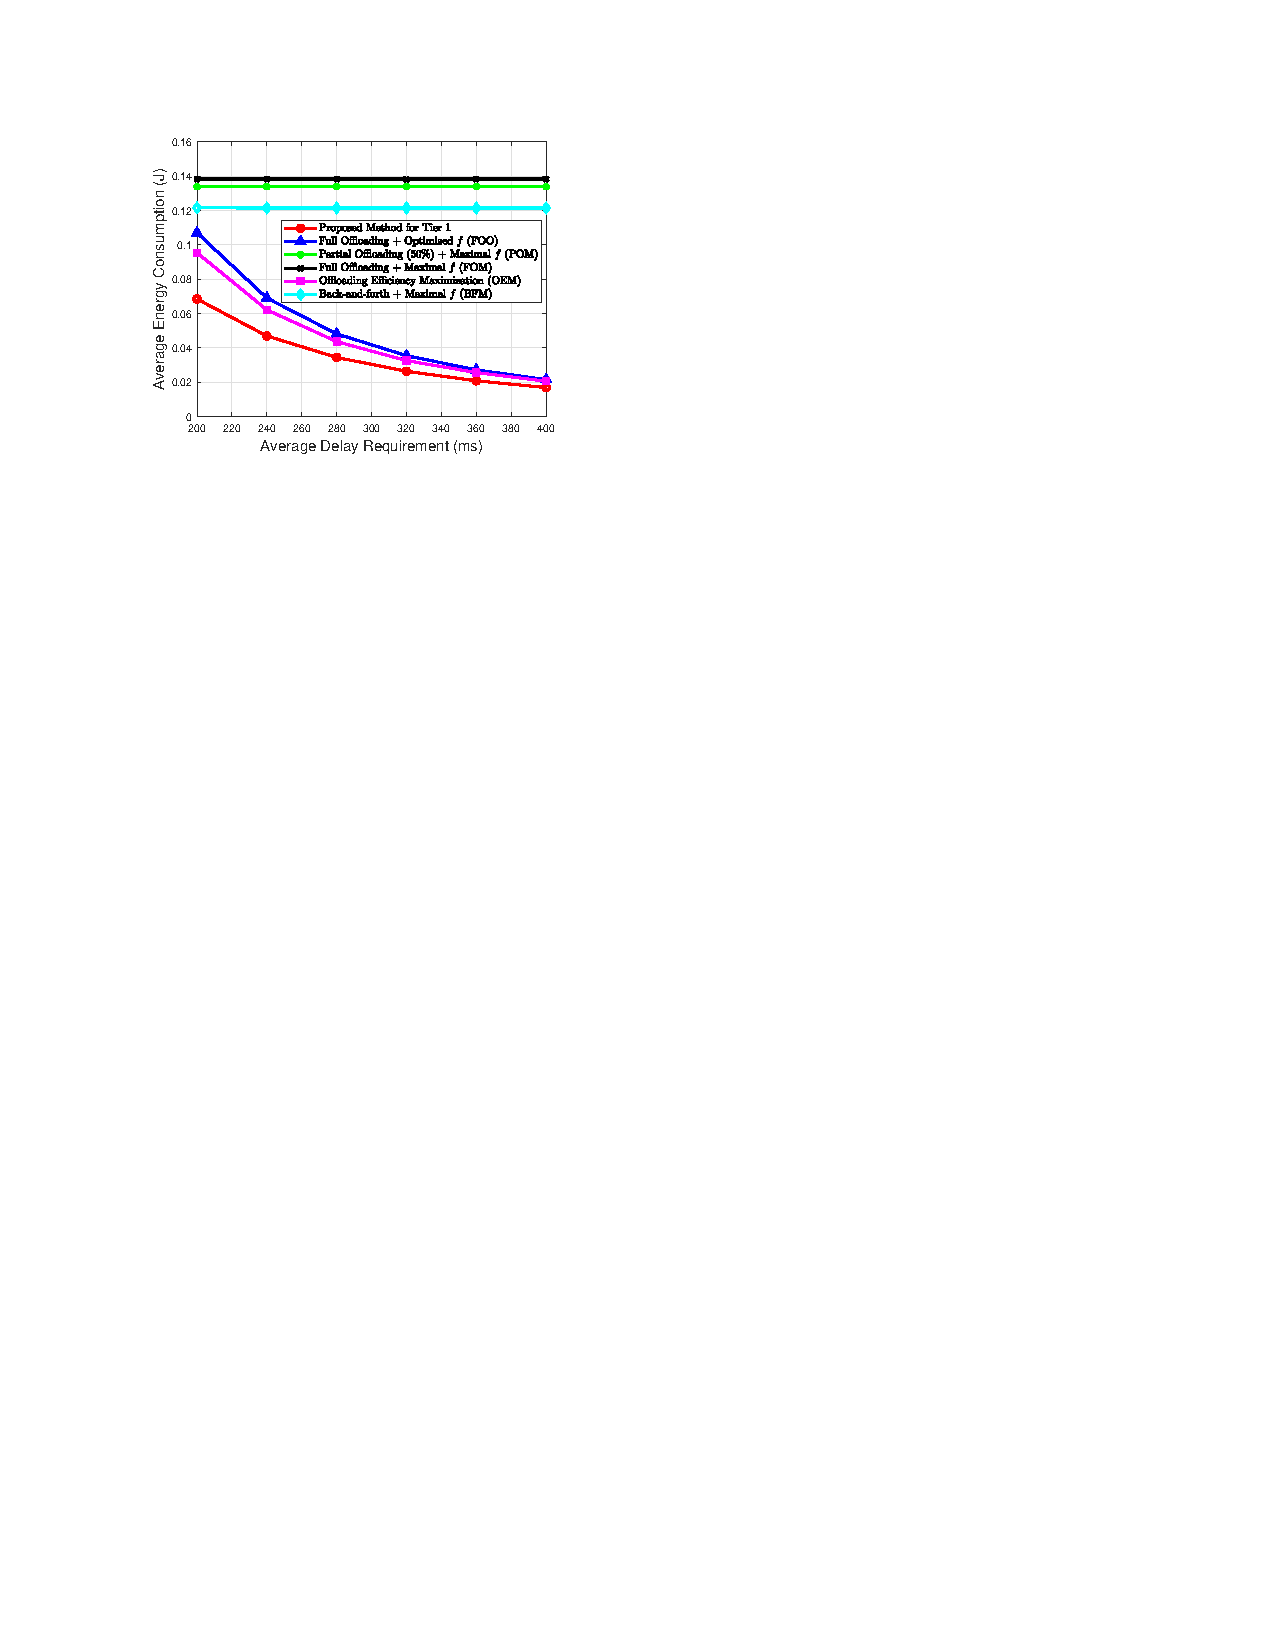
\includegraphics[width=3 in]{Figures/Tier_1_E1}
\caption{Average energy consumption for different methods under varying task delay requirement.}
\label{fig_3}
\end{figure}

\begin{figure}[!t]
\centering
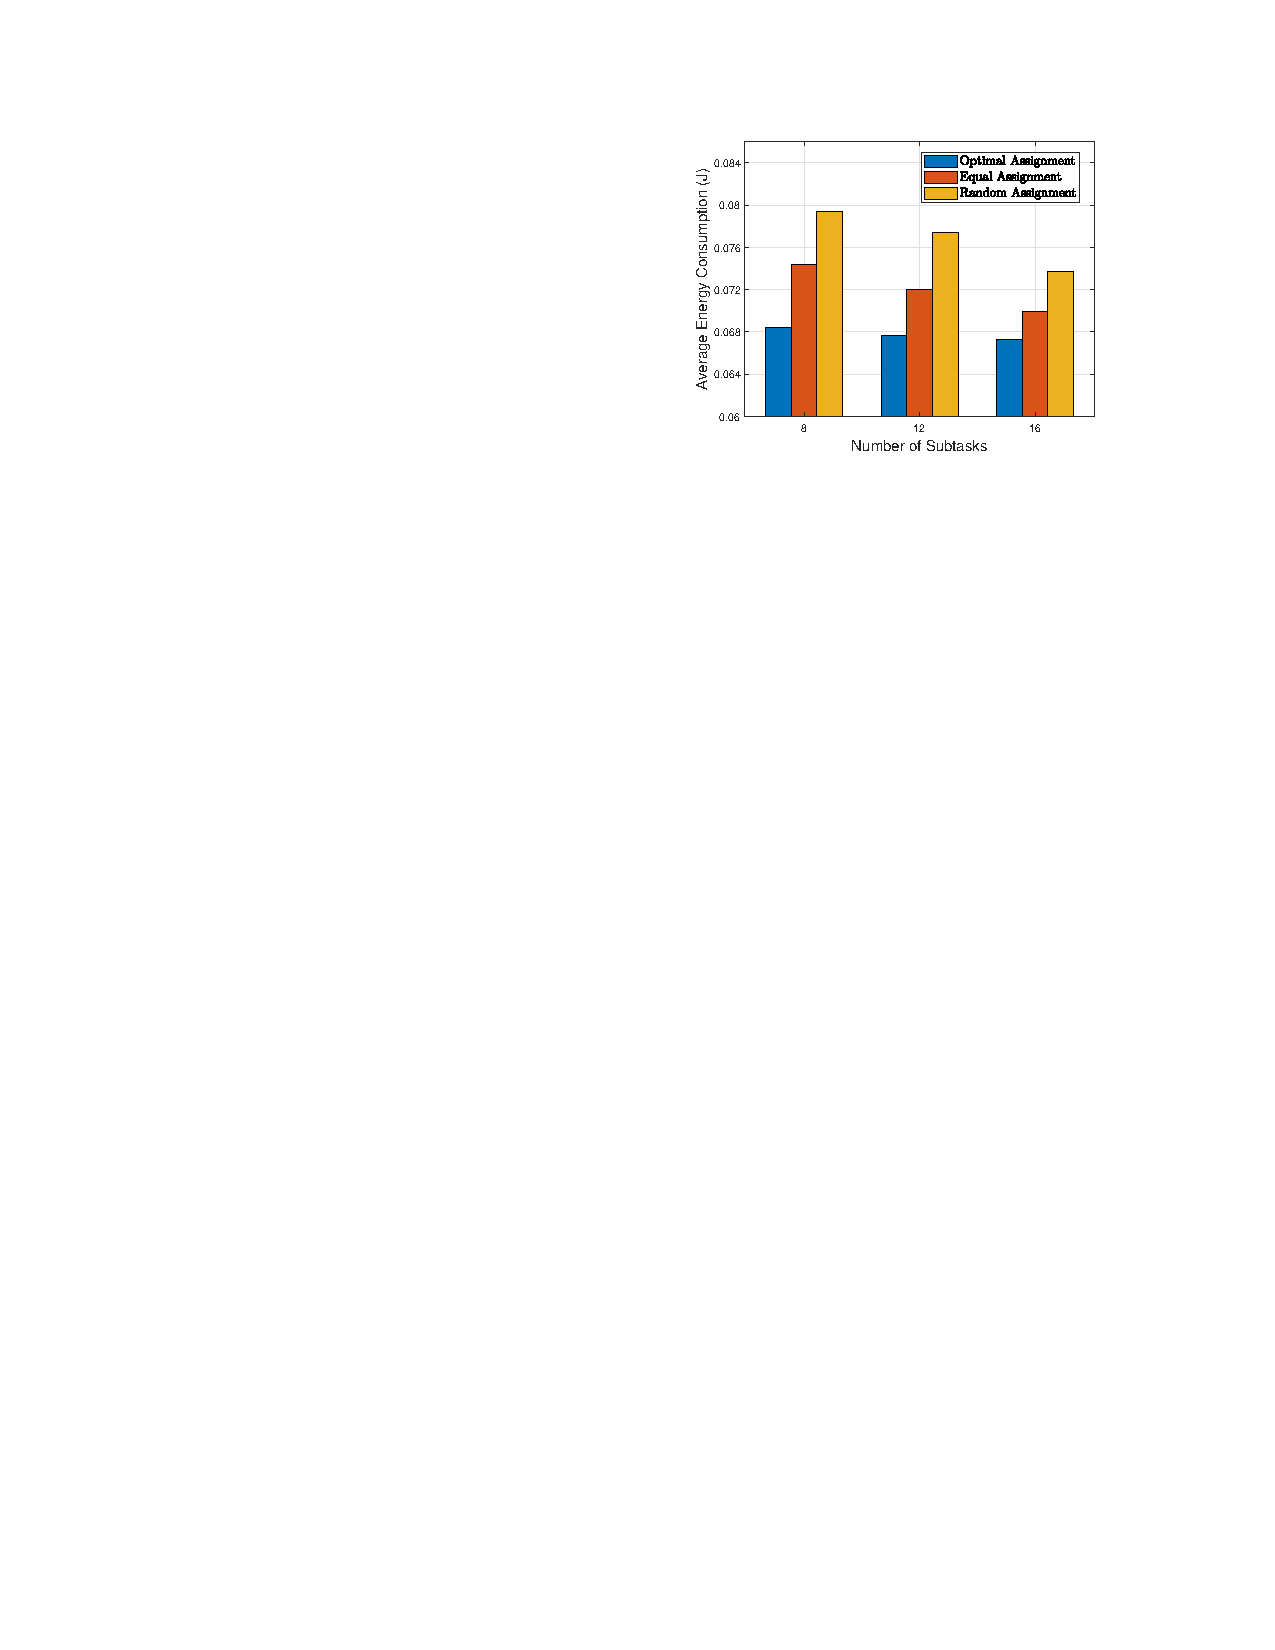
\includegraphics[width=3.0 in]{Figures/Tier_1_E2}
\caption{Average energy consumption with varying subtask structure.}
\label{fig_4}
\end{figure}




\textbf{(1) AEC for different methods under varying task delay requirement:} Fig. 3 shows the AEC when adopting diverse methods with the constraint of different task delay requirements. We compare the performance of the proposed method with the following five algorithms:

\begin{itemize}

\item \textit{Full Offloading $+$ Optimized CPU Frequency $f$ (FOO)}: NV offloads all subtasks to its HV and HV adopts the CPU frequency optimized by the proposed method.

\item \textit{Partial Offloading $(50\%)$ $+$ Maximal $f$ (POM)}: Each pair of NV and HV undertakes half of the subtasks and utilizes maximal CPU frequency.

\item \textit{Full Offloading $+$ Maximal $f$ (FOM)}: NV offloads all subtasks to HV and HV adopts maximal CPU frequency.

\item \textit{Offloading Efficiency Maximization (OEM)}: The dependency-aware task offloading and resource allocation scheme that aims to maximize offloading efficiency proposed in \cite{ref22}.

\item \textit{Back-and-forth $+$ Maximal $f$ (BFM)}: The ratio of computational workload assigned to NV and HV is as close to the ratio of their computing capacity as possible. They compute in a back-and-forth manner using their maximal CPU frequency.

\end{itemize}

The experimental results validate that the proposed method consistently achieves the minimum AEC across varying task delay requirements, demonstrating its effectiveness and robustness under diverse delay constraints. Moreover, the advantages of the proposed method are increasingly significant as the delay requirements become more stringent. In addition, we can observe that the methods utilizing the maximal CPU frequency $f$ (i.e., FOM, POM, and BFM) result in significantly higher AEC than methods with optimized $f$ and FOM causes the highest AEC among them. This is because the computation energy consumption is proportional to the square of CPU frequency. Hence, it will be significantly amplified when maximum frequency is adopted. FOM employs the maximal CPU frequency of HV to compute all subtasks, thereby rendering it the most energy-consuming method. It is also worth noting that, for FOM, POM, and BFM, the computation energy consumption is deterministic due to the use of fixed CPU frequency. Varying delay requirements only affect the communication energy consumption with minor portion. As a result, their AEC exhibits insignificant variation with changes in delay requirements. In contrast, for the remaining three methods, a more relaxed latency requirement implies that vehicles are allowed to compute at a slower speed, thus achieving lower computation energy consumption.

\begin{figure}[!t]
\centering
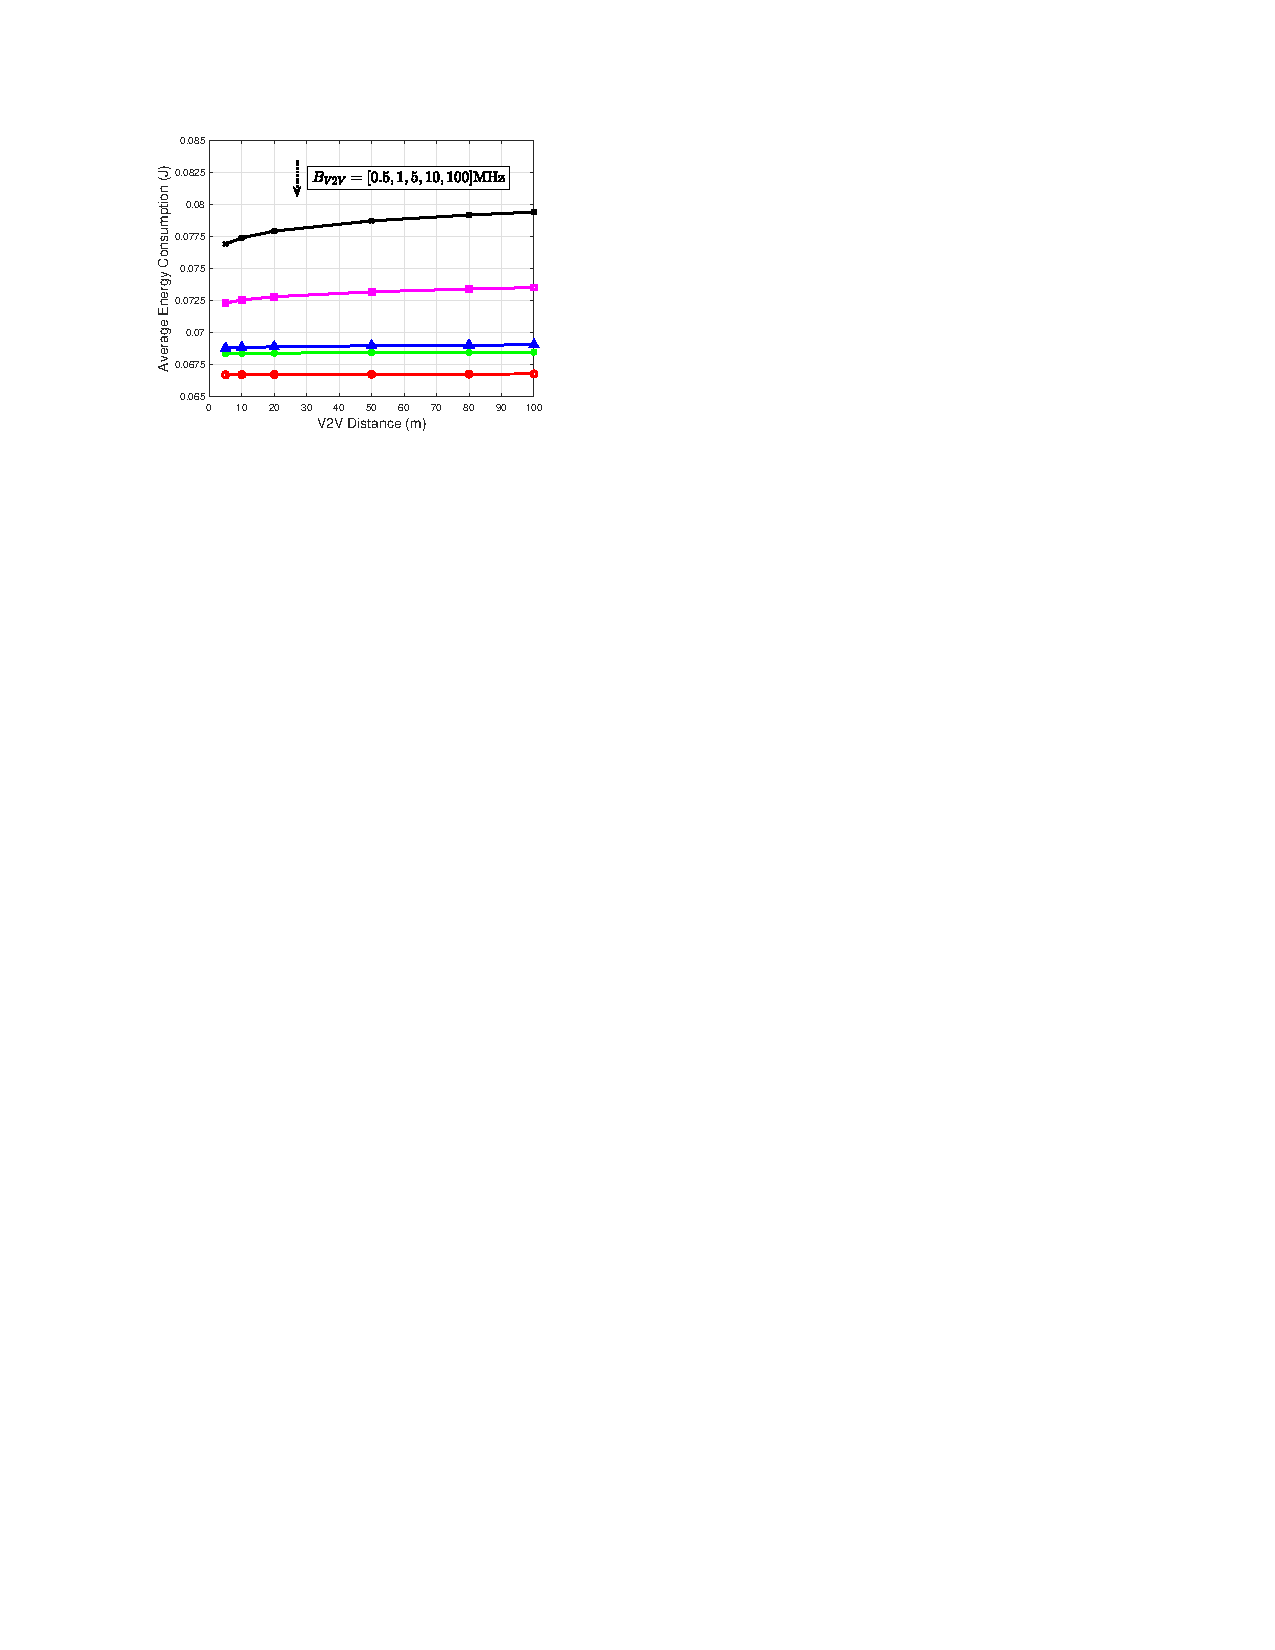
\includegraphics[width=2.8 in]{Figures/Tier_1_E3}
\caption{Impact of V2V bandwidth and distance on average energy consumption.}
\label{fig_5}
\end{figure}

\begin{figure}[!t]
\centering
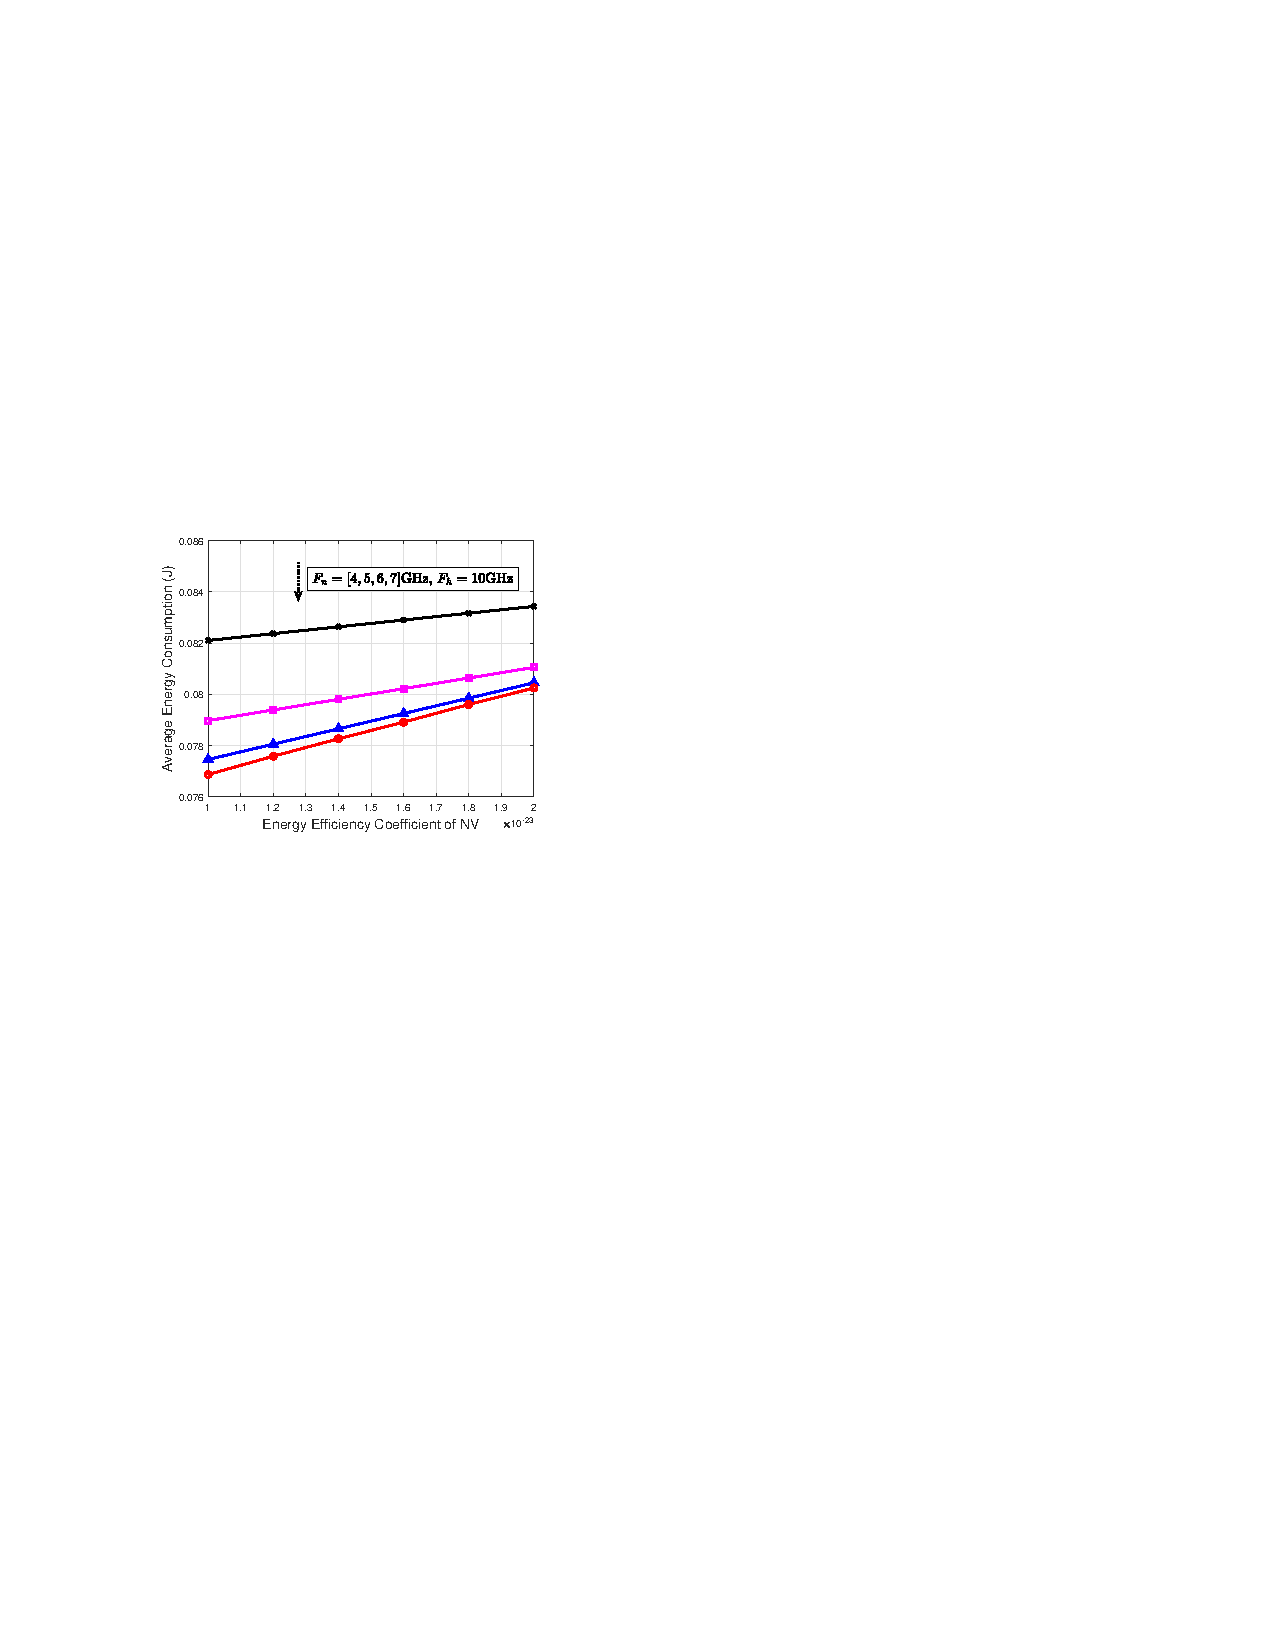
\includegraphics[width=2.8 in]{Figures/Tier_1_E4}
\caption{Impact of computing capacity and energy efficiency coefficient of NV on average energy consumption.}
\label{fig_6}
\end{figure}


\textbf{(2) Impact of subtask structure:} In Fig. 4, we fix the total input data size and computational workloads of the application tasks and change the number of subtasks by further splitting some of them. For a fixed subtask number, we adopt different task offloading decisions (i.e., the optimal, equal, and random assignment). Undoubtedly, optimal offloading decision always has the best performance, since it always selects the offloading decision associated with the lowest AEC. Random assignment significantly increases AEC since it undergoes high uncertainty. The performance of equal assignment lies between the above two. Moreover, from a general perspective, we can tell the pattern that the finer the division of subtasks, the better the Tier-1 method will work. Therefore, for a certain offloading method, the AEC will decrease with the number of subtasks. However, this conclusion is drawn based on extensive experimental results and is applicable to the most cases, and exceptions may exist for certain special scenarios.


\textbf{(3) Impact of V2V bandwidth and distance between NV and HV:} In the scenario of Fig. 5, we set $B_{V2V}$ as $0.5 MHz$, $1 MHz$, $5 MHz$, $10 MHz$ and $100 MHz$. It can be observed that the AEC continues to decrease as $B_{V2V}$ increases, which can be interpreted from two perspectives: On the one hand, to achieve the same link data rate, the larger the $B_{V2V}$, the less transmit power needed. On the other hand, for a fixed transmit power, a larger $B_{V2V}$ will increase the link data rate. Hence, the transmission delay is reduced. Thus, there is more time left for the computation part for vehicles, which means they can compute with lower CPU frequency. This is less energy-consuming. Plus, for a fixed $B_{V2V}$, the longer the distance between two vehicles, the higher the AEC due to the need for a larger transmit power. However, the increase is not significant, since transmission energy consumption accounts for a small proportion compared to computation energy consumption.

\begin{figure}[!t]
\centering
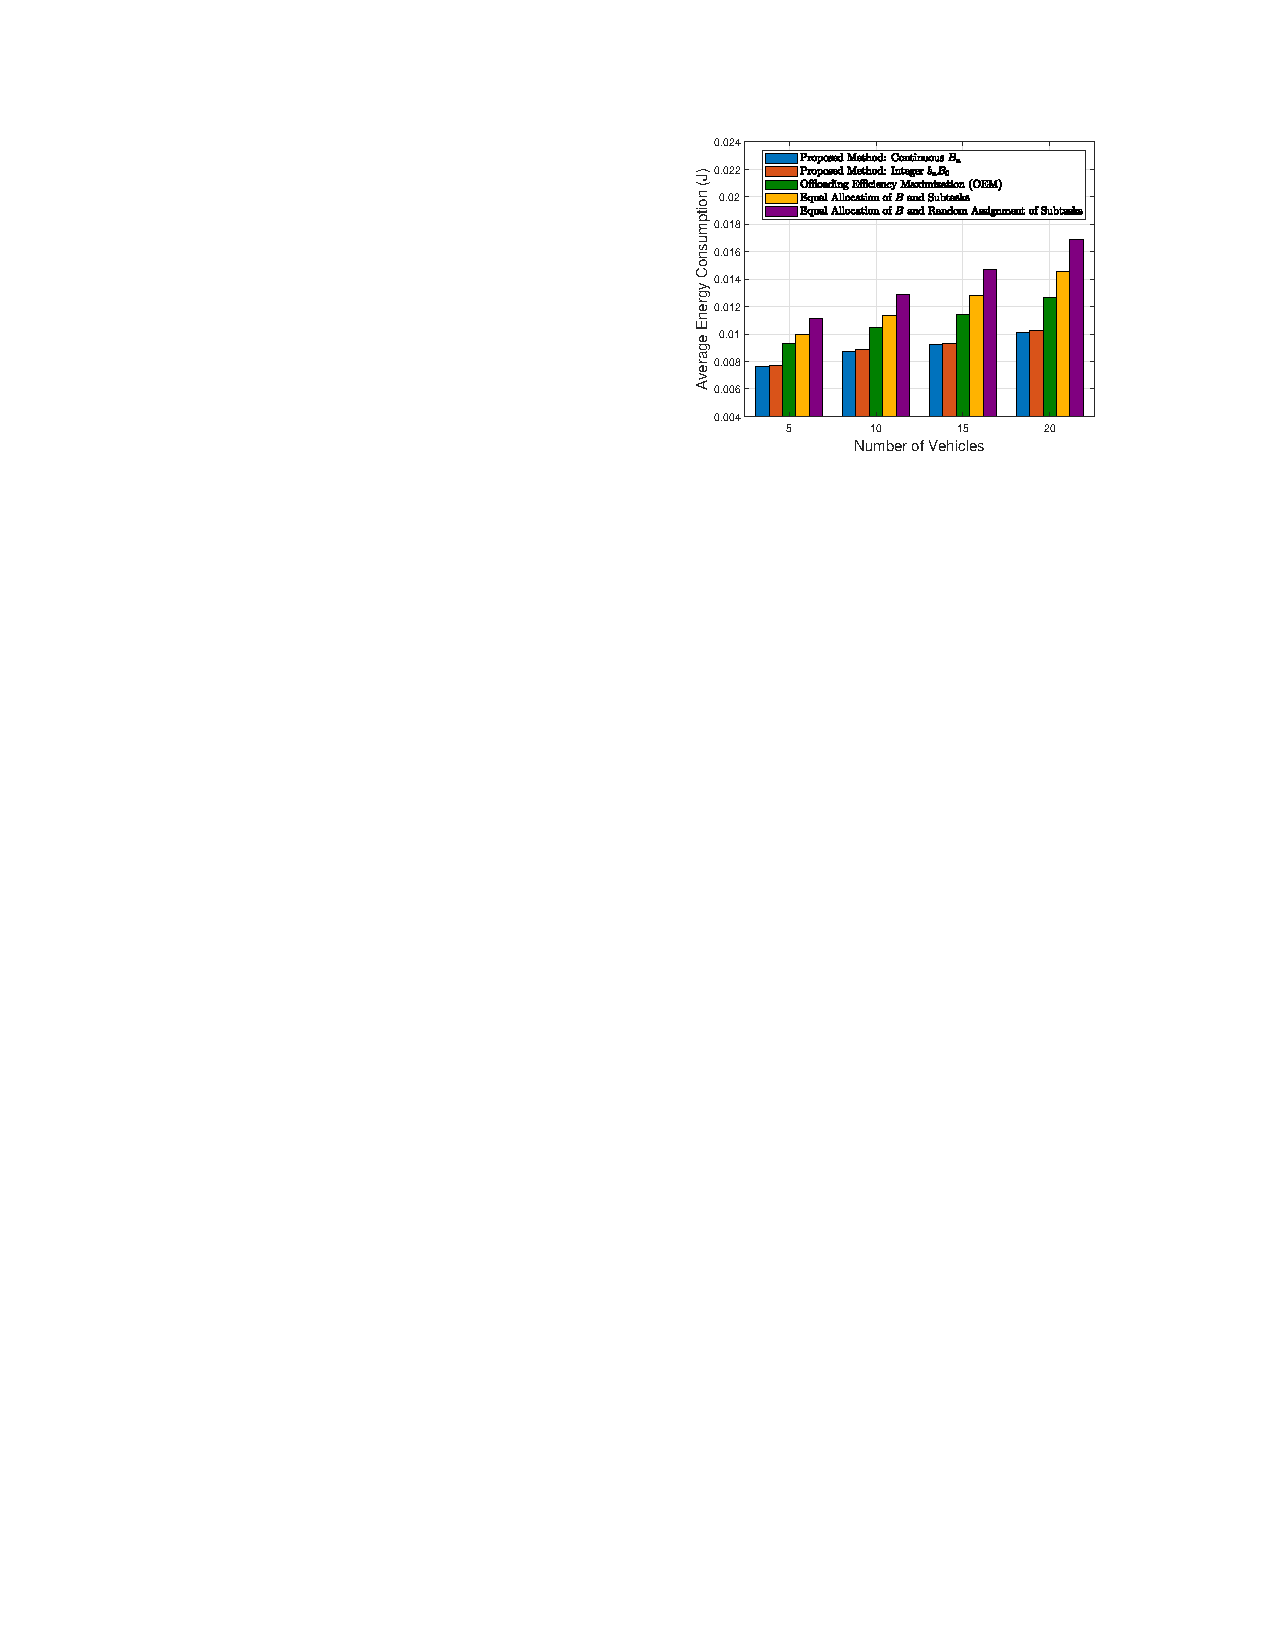
\includegraphics[width=2.8 in]{Figures/Tier_2_E1}
\caption{Average energy consumption for different methods.}
\label{fig_7}
\end{figure}

\begin{figure}[!t]
\centering
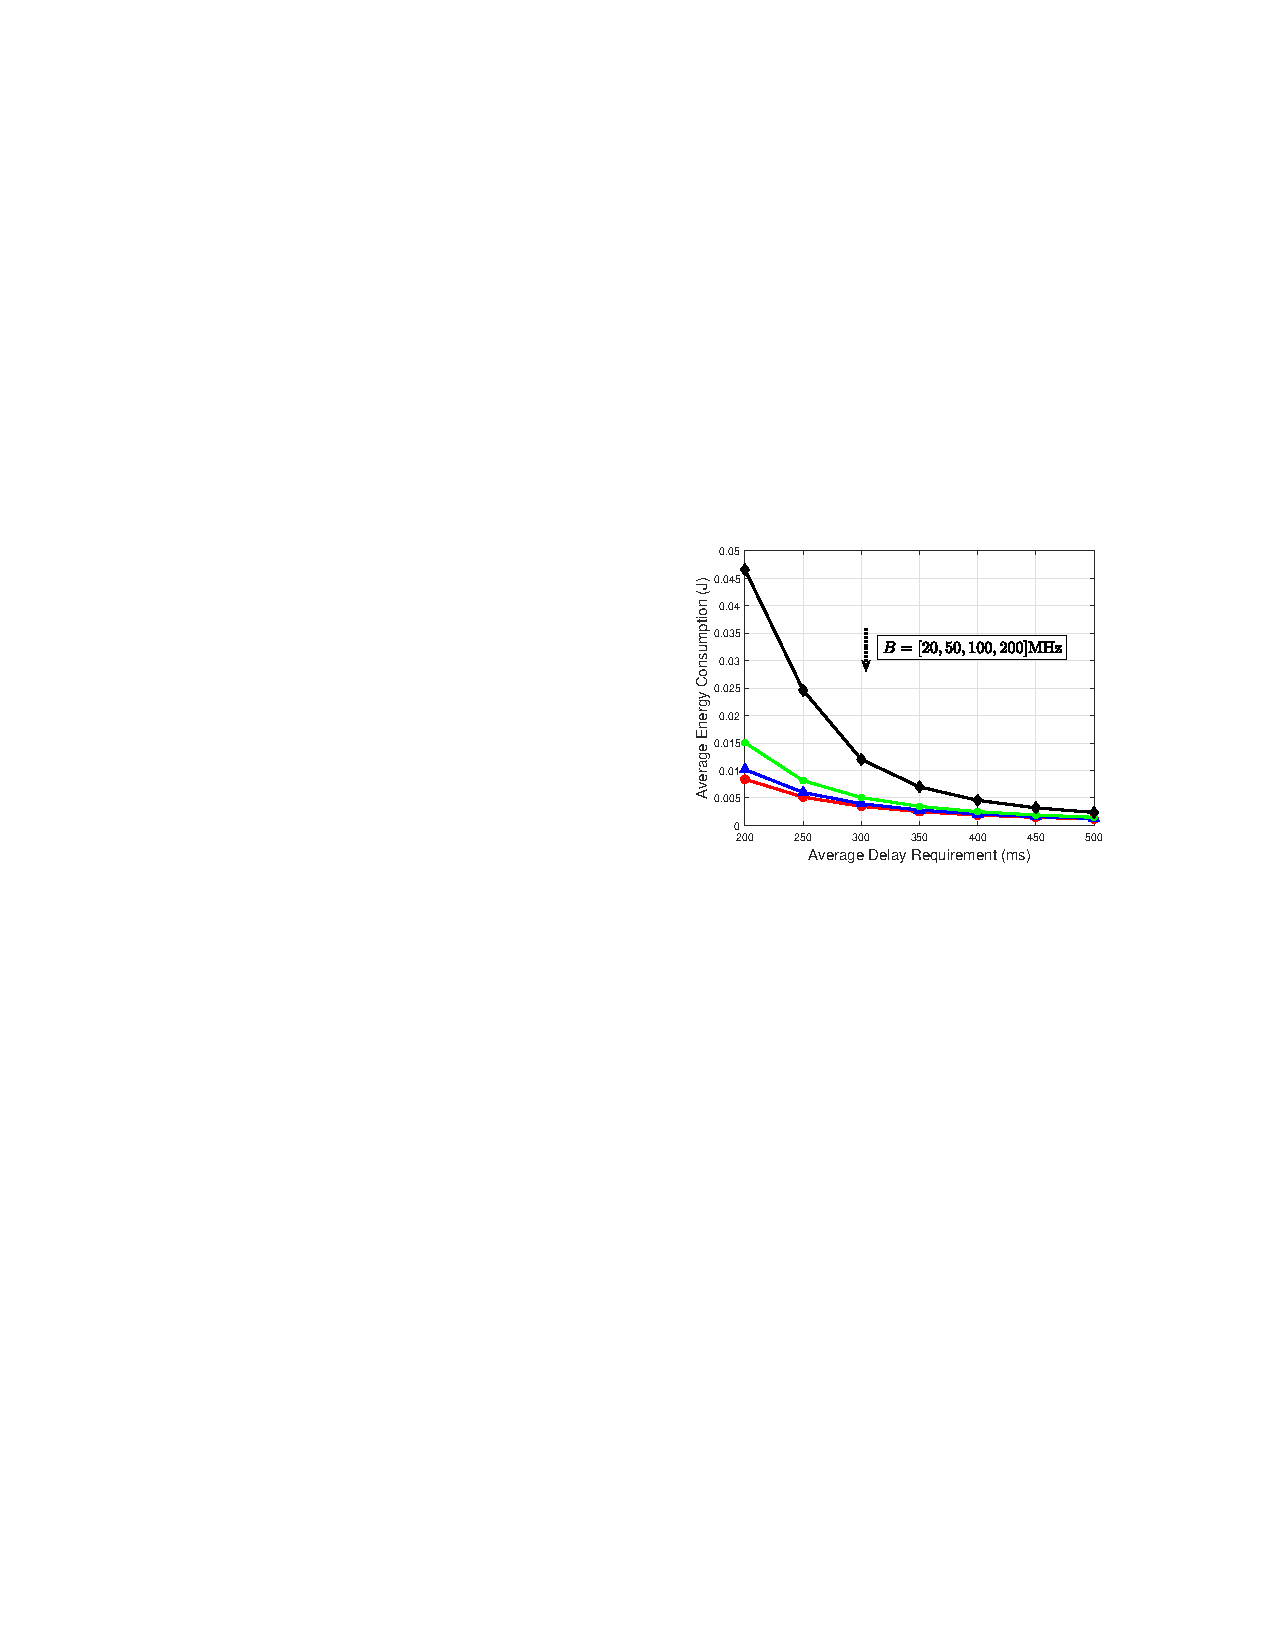
\includegraphics[width=2.8 in]{Figures/Tier_2_E2}
\caption{Impact of system bandwidth on average energy consumption.}
\label{fig_8}
\end{figure}

\begin{figure}[!t]
\centering
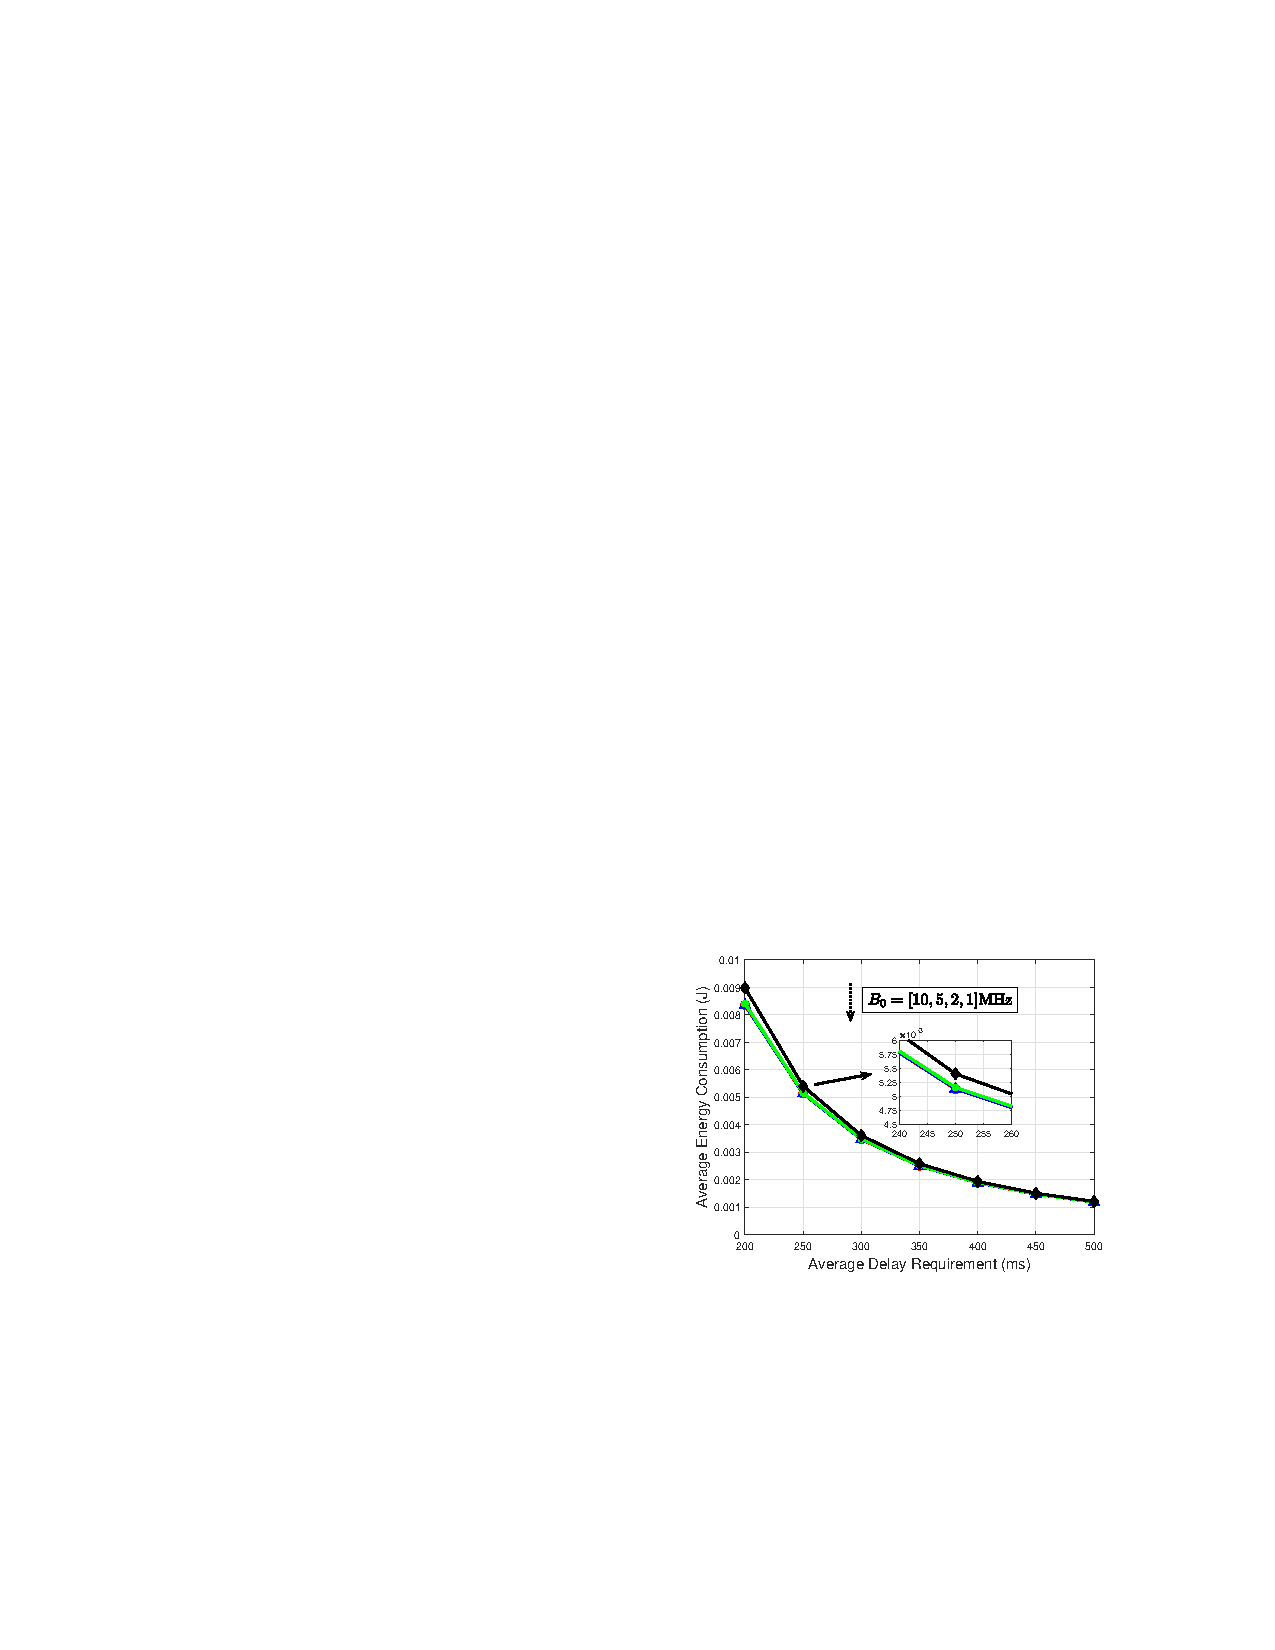
\includegraphics[width=2.8 in]{Figures/Tier_2_E3}
\caption{Impact of subchannel bandwidth on average energy consumption.}
\label{fig_9}
\end{figure}

\textbf{(4) Impact of computing capacity and energy efficiency coefficient of NV:} In Fig. 6, we fix the maximal computing resource of HV as $10 GHz$ and change that of NV as $4 GHz$, $5 GHz$, $6 GHz$ and $7 GHz$, respectively. We can conclude that the closer the computing capacity of NV to that of HV, the less the AEC. Since if NV can compute faster, the time left for HV will not be that tight so that HV can compute more slowly. The increase in NV's computation energy will be smaller than the decrease in HV, leading to less total energy consumption. For a fixed computing capacity of NV and HV, the AEC will increase with the energy efficiency coefficient (i.e., $\kappa$) of the vehicle. Additionally, when the computing capacity of a vehicle is enhanced, its computation energy consumption becomes more sensitive to $\kappa$, since the workload it undertakes also increases correspondingly.


\subsection{Experiment for RSU Tier}

The service range of RSU is set as 200 m according to \cite{ref31}. Similarly to Tier-1, the energy efficiency coefficients of RSUs are also configured within the range of $[1, 2]\times 10^{-23}$, and their maximal computing resources are set within the interval of $[60,120] GHz$. In terms of a series of parameters related to communication, we set the communication setup delay to $0.1 ms$, $E_0=10^{-5} J$ and $\tau_0=10^{-5} ms$. These parameters can be easily adjusted in practical applications. The AEC is normalized by the default system bandwidth (i.e., $100 MHz$).

Based on the current setup, it takes several seconds for each vehicle to traverse the service range of an RSU, which has already significantly exceeded the task delay requirement in this study (i.e., on the order of hundreds of milliseconds). Therefore, to achieve multi-RSU cooperation and also spatial practicality, we consider the scenario of two RSUs cooperation in this experiment. This method is also scalable to scenarios with a larger number of RSUs.


\textbf{(1) AEC for different methods with diverse number of NV:} Fig. 7 depicts the AEC with following five different methods under varying number of NV. 

\begin{itemize}

\item \textit{Proposed Method: Continuous $B_n$}: The proposed method with treating $B_n$ as continuous variables.

\item \textit{Proposed Method: Integer $b_n B_0$}: The proposed method with allocating $b_n$ subchannels to each V2I link (i.e., subchannel bandwidth is $1 MHz$).

\item \textit{Offloading Efficiency Maximization (OEM)}: The offloading efficiency maximization scheme proposed in \cite{ref22}.

\item \textit{Equal Allocation of $B$ and Subtasks}: Equal bandwidth allocation for each V2I uplink and equal subtask assignment for each RSU.

\item \textit{Equal Allocation of $B$ and Random Assignment of Subtasks}: Equal bandwidth allocation for each V2I uplink and random subtask assignment for each RSU.

\end{itemize}


All four methods other than OEM utilize optimal computing resource allocation to prevent excessive energy consumption by powerful edge servers. The proposed method with continuous $B_n$ demonstrates the best performance as it achieves optimality for all optimization variables. Discretizing the variable $B_n$, as in the second method, results in a slight increase in AEC due to the subtle deviation from the optimal continuous solution, but the performance degradation is minimal. OEM shows a noticeable increase in AEC compared to the first two methods. The strategy of equally allocating $B$ and subtasks undergoes a significant performance degradation compared with proposed method, since it exhibits an obvious disadvantage when encountering unbalanced workload distribution among subtasks. The method represented by purple column performs the worst, as the random assignment of subtasks introduces greater uncertainty. Additionally, the AEC gradually increases with the number of NVs, as more NVs intensify competition for bandwidth resources, resulting in higher transmission energy consumption and delay. Furthermore, RSUs have less time for computation, leading to their higher CPU frequency and increased energy consumption.


\textbf{(2) Impact of system bandwidth and subchannel bandwidth:} In the scenario of Fig. 8, we change the system bandwidth as $20 MHz$, $50 MHz$, $100 MHz$ and $200 MHz$, respectively. It can be concluded that a higher system bandwidth can reduce AEC since it improves the data rate of V2I uplinks, saving more time for computation. Fig. 8 also illustrates that the looser the average delay requirement, the lower the AEC. Because for both data transmission and task computation, more ample time means lower working power, which will reduce energy consumption.

Fig. 9 shows the impact of the granularity of subchannel division on AEC. With the increase of subchannel bandwidth, the AEC shows an upward trend. This is because the coarser the granularity of partitioning, the more the bandwidth allocation policy deviates from the optimal continuous solution, hence the worse performance. However, within an appropriate range, the impact of partitioning granularity is not very significant since after discretizing the continuous $B_n^*$, we do not reoptimize other variables based on it again, which would not destroy the already optimal variables. Additionally, transmission energy accounts for a small portion in the total energy consumption. Thus, the impact of bandwidth allocation deviation relative to the optimal solution on AEC appears to be subtle overall.


%%%%%%%%%%%%%%%%%%%%%%%%%%%%%%%%%%%%%%%%%%%%%%%%%%%%%%%%%%%%%%%%%%%%%%%%%%%%%%%%%%%%

\section{Conclusions}

In this article, we have proposed a V2X communication-empowered multi-tier task offloading mechanism dedicated for the applications with sequential subtasks in vehicular networks. The proposed NV-HV matching scheme can effectively cope with highly variable speed, spatial distribution, and computing capabilities of vehicles, while maximizing the number of matched NVs in the vehicle tier. The formulated problem of joint task offloading decisions, communication, and computing resources allocation optimization in each tier can be efficiently solved by KKT conditions algorithm, which ensures maximization of system energy efficiency while guaranteeing timely task completion. We further designed a two-step method to allocate subchannels for each V2I link, achieving performance that is close to the optimal continuous solution. Extensive experiments were conducted to demonstrate the performance superiority of the proposed method over baseline methods and evaluate its responsiveness to diverse system parameters. These results provide valuable insights and contribute to the development of efficient and reliable sequential task offloading schemes in MEC-enabled vehicular networks.



\begin{thebibliography}{10}
\bibliographystyle{IEEEtran}

\bibitem{ref1}
Y. Zhang, M. Xu, Y. Qin, M. Dong, L. Gao and E. Hashemi, ``MILE: Multiobjective Integrated Model Predictive Adaptive Cruise Control for Intelligent Vehicle," \textit{IEEE Transactions on Industrial Informatics}, vol. 19, no. 7, pp. 8539-8548, July 2023.

\bibitem{ref2}
X. Cheng, D. Duan, S. Gao and L. Yang, ``Integrated Sensing and Communications (ISAC) for Vehicular Communication Networks (VCN)," \textit{IEEE Internet of Things Journal}, vol. 9, no. 23, pp. 23441-23451, 1 Dec.1, 2022.

\bibitem{ref3}
X. Cheng, S. Gao and L. Yang, \textit{mmWave Massive MIMO Vehicular Communications}, Cham, Switzerland: Springer, 2022.


\bibitem{ref4}
X. Zheng, Y. Li, D. Duan, L. Yang, C. Chen and X. Cheng, ``Multivehicle Multisensor Occupancy Grid Maps (MVMS-OGM) for Autonomous Driving," \textit{IEEE Internet of Things Journal}, vol. 9, no. 22, pp. 22944-22957, 15 Nov.15, 2022.


\bibitem{ref5}
D. Katare, D. Perino, J. Nurmi, M. Warnier, M. Janssen and A. Y. Ding, ``A Survey on Approximate Edge AI for Energy Efficient Autonomous Driving Services," \textit{IEEE Communications Surveys \& Tutorials}, vol. 25, no. 4, pp. 2714-2754, Fourthquarter 2023.


\bibitem{ref6}
D. Roy, Y. Li, T. Jian, P. Tian, K. Chowdhury and S. Ioannidis, ``Multi-Modality Sensing and Data Fusion for Multi-Vehicle Detection," \textit{IEEE Transactions on Multimedia}, vol. 25, pp. 2280-2295, 2023.

\bibitem{ref7}
X. Cheng, J. Zhou, P. Liu, X. Zhao and H. Wang, ``3D Vehicle Object Tracking Algorithm Based on Bounding Box Similarity Measurement," \textit{IEEE Transactions on Intelligent Transportation Systems}, vol. 24, no. 12, pp. 15844-15854, Dec. 2023.

\bibitem{ref8}
Y. Mao, C. You, J. Zhang, K. Huang and K. B. Letaief, ``A Survey on Mobile Edge Computing: The Communication Perspective," \textit{IEEE Communications Surveys \& Tutorials}, vol. 19, no. 4, pp. 2322-2358, Fourthquarter 2017.

\bibitem{ref9}
W. Fan et al., ``Collaborative Service Placement, Task Scheduling, and Resource Allocation for Task Offloading With Edge-Cloud Cooperation," \textit{IEEE Transactions on Mobile Computing}, vol. 23, no. 1, pp. 238-256, Jan. 2024.

\bibitem{ref10}
J. Yan, Q. Lu and G. B. Giannakis, ``Bayesian Optimization for Online Management in Dynamic Mobile Edge Computing," \textit{IEEE Transactions on Wireless Communications}, vol. 23, no. 4, pp. 3425-3436, April 2024.


\bibitem{ref11}
H. Jiang, X. Dai, Z. Xiao and A. Iyengar, ``Joint Task Offloading and Resource Allocation for Energy-Constrained Mobile Edge Computing," \textit{IEEE Transactions on Mobile Computing}, vol. 22, no. 7, pp. 4000-4015, 1 July 2023.

\bibitem{ref12}
S. Chen, W. Li, J. Sun, P. Pace, L. He and G. Fortino, ``An Efficient Collaborative Task Offloading Approach Based on Multi-Objective Algorithm in MEC-Assisted Vehicular Networks," \textit{IEEE Transactions on Vehicular Technology}, doi: 10.1109/TVT.2025.3543412.

\bibitem{ref13}
Q. Wu, S. Wang, H. Ge, P. Fan, Q. Fan and K. B. Letaief, ``Delay-Sensitive Task Offloading in Vehicular Fog Computing-Assisted Platoons," \textit{IEEE Transactions on Network and Service Management}, vol. 21, no. 2, pp. 2012-2026, April 2024.

\bibitem{ref14}
L. Yin, J. Luo, C. Qiu, C. Wang and Y. Qiao, ``Joint Task Offloading and Resources Allocation for Hybrid Vehicle Edge Computing Systems," \textit{IEEE Transactions on Intelligent Transportation Systems}, vol. 25, no. 8, pp. 10355-10368, Aug. 2024.

\bibitem{ref15}
H. Guo, L. -l. Rui and Z. -p. Gao, ``V2V Task Offloading Algorithm with LSTM-based Spatiotemporal Trajectory Prediction Model in SVCNs," \textit{IEEE Transactions on Vehicular Technology}, vol. 71, no. 10, pp. 11017-11032, Oct. 2022.

\bibitem{ref16}
X. Wang, S. Wang, X. Gao, Z. Qian and Z. Han, ``AMTOS: An ADMM-Based Multilayer Computation Offloading and Resource Allocation Optimization Scheme in IoV-MEC System," \textit{IEEE Internet of Things Journal}, vol. 11, no. 19, pp. 30953-30964, 1 Oct.1, 2024.

\bibitem{ref17}
W. Shu, X. Feng and C. Guo, ``An Adaptive Alternating Direction Method of Multipliers for Vehicle-to-Everything Computation Offloading in Cloud–Edge Collaborative Environment," \textit{IEEE Internet of Things Journal}, vol. 11, no. 22, pp. 35802-35811, 15 Nov.15, 2024.

\bibitem{ref18}
Y. Wu, X. Zhu, J. Fei and H. Xu, ``A Novel Joint Optimization Method of Multi-Agent Task Offloading and Resource Scheduling for Mobile Inspection Service in Smart Factory," \textit{IEEE Transactions on Vehicular Technology}, vol. 73, no. 6, pp. 8563-8575, June 2024.

\bibitem{ref19}
H. Zhang, X. Liu, Y. Xu, D. Li, C. Yuen and Q. Xue, ``Partial Offloading and Resource Allocation for MEC-Assisted Vehicular Networks," \textit{IEEE Transactions on Vehicular Technology}, vol. 73, no. 1, pp. 1276-1288, Jan. 2024.

\bibitem{ref20}
S. Li, W. Sun, Q. Ni and Y. Sun, ``Road Side Unit-Assisted Learning-Based Partial Task Offloading for Vehicular Edge Computing System," \textit{IEEE Transactions on Vehicular Technology}, vol. 73, no. 4, pp. 5546-5555, April 2024.

\bibitem{ref21}
N. Fofana, A. B. Letaifa and A. Rachedi, ``Intelligent Task Offloading in Vehicular Networks: A Deep Reinforcement Learning Perspective," \textit{IEEE Transactions on Vehicular Technology}, vol. 74, no. 1, pp. 201-216, Jan. 2025.

\bibitem{ref22}
Q. Shen, B. -J. Hu and E. Xia, ``Dependency-Aware Task Offloading and Service Caching in Vehicular Edge Computing," \textit{IEEE Transactions on Vehicular Technology}, vol. 71, no. 12, pp. 13182-13197, Dec. 2022.

\bibitem{ref23}
H. Liu, W. Huang, D. I. Kim, S. Sun, Y. Zeng and S. Feng, ``Towards Efficient Task Offloading With Dependency Guarantees in Vehicular Edge Networks Through Distributed Deep Reinforcement Learning," \textit{IEEE Transactions on Vehicular Technology}, vol. 73, no. 9, pp. 13665-13681, Sept. 2024.

\bibitem{ref24}
L. Zhao et al., ``MESON: A Mobility-Aware Dependent Task Offloading Scheme for Urban Vehicular Edge Computing," \textit{IEEE Transactions on Mobile Computing}, vol. 23, no. 5, pp. 4259-4272, May 2024.

\bibitem{ref25}
X. Dai et al., ``A Learning-Based Approach for Vehicle-to-Vehicle Computation Offloading," \textit{IEEE Internet of Things Journal}, vol. 10, no. 8, pp. 7244-7258, 15 April15, 2023.

\bibitem{ref26}
P. Dai, Y. Huang, K. Hu, X. Wu, H. Xing and Z. Yu, ``Meta Reinforcement Learning for Multi-Task Offloading in Vehicular Edge Computing," \textit{IEEE Transactions on Mobile Computing}, vol. 23, no. 3, pp. 2123-2138, March 2024.

\bibitem{ref27}
H. Zhou, W. Xu, J. Chen and W. Wang, ``Evolutionary V2X Technologies Toward the Internet of Vehicles: Challenges and Opportunities," \textit{Proceedings of the IEEE}, vol. 108, no. 2, pp. 308-323, Feb. 2020.

\bibitem{ref28}
R. M. Corless, G. H. Gonnet, D. E. G. Hare, D. J. Jeffrey, and D. E. Knuth, ``On the Lambert W function,” \textit{Adv. Comput. Math.}, vol. 5, no. 1, pp. 329–359, Dec. 1996.

\bibitem{ref29}
Y. Fan, S. Gao, D. Duan, X. Cheng and L. Yang, ``Radar Integrated MIMO Communications for Multi-Hop V2V Networking," \textit{IEEE Wireless Communications Letters}, vol. 12, no. 2, pp. 307-311, Feb. 2023.

\bibitem{ref30}
M. Z. Alam and A. Jamalipour, ``Multi-Agent DRL-Based Hungarian Algorithm (MADRLHA) for Task Offloading in Multi-Access Edge Computing Internet of Vehicles (IoVs)," \textit{IEEE Transactions on Wireless Communications}, vol. 21, no. 9, pp. 7641-7652, Sept. 2022.

\bibitem{ref31}
Z. Xiao, J. Shu, H. Jiang, G. Min, H. Chen and Z. Han, ``Perception Task Offloading With Collaborative Computation for Autonomous Driving," \textit{IEEE Journal on Selected Areas in Communications}, vol. 41, no. 2, pp. 457-473, Feb. 2023.

\bibitem{ref32}
A. Krizhevsky, I. Sutskever, and G. E. Hinton, ``ImageNet classification with deep convolutional neural networks,” \textit{Proc. Int. Conf. Adv. Neural Inf. Process. Syst.}, pp. 1097–1105, Jan. 2012.


% \bibitem{ref18}
% H. Tang, H. Wu, G. Qu and R. Li, ``Double Deep Q-Network Based Dynamic Framing Offloading in Vehicular Edge Computing," \textit{IEEE Transactions on Network Science and Engineering}, vol. 10, no. 3, pp. 1297-1310, 1 May-June 2023.

% \bibitem{ref19}
% P. Dai, Y. Huang, K. Hu, X. Wu, H. Xing and Z. Yu, ``Meta Reinforcement Learning for Multi-Task Offloading in Vehicular Edge Computing," \textit{IEEE Transactions on Mobile Computing}, vol. 23, no. 3, pp. 2123-2138, March 2024.

% \bibitem{ref20}
% Y. -J. Ku, S. Baidya and S. Dey, ``Uncertainty-Aware Task Offloading for Multi-Vehicle Perception Fusion Over Vehicular Edge Computing," \textit{IEEE Transactions on Vehicular Technology}, vol. 72, no. 11, pp. 14906-14923, Nov. 2023.

% \bibitem{ref21}
% X. Dai et al., ``A Learning-Based Approach for Vehicle-to-Vehicle Computation Offloading," \textit{IEEE Internet of Things Journal}, vol. 10, no. 8, pp. 7244-7258, 15 April15, 2023.

% \bibitem{ref22}
% Z. Wang, D. Zhao, M. Ni, L. Li and C. Li, ``Collaborative Mobile Computation Offloading to Vehicle-Based Cloudlets," \textit{IEEE Transactions on Vehicular Technology}, vol. 70, no. 1, pp. 768-781, Jan. 2021.

% \bibitem{ref23}
% Z. Wang, Z. Zhong, D. Zhao and M. Ni, ``Vehicle-Based Cloudlet Relaying for Mobile Computation Offloading," \textit{IEEE Transactions on Vehicular Technology}, vol. 67, no. 11, pp. 11181-11191, Nov. 2018.

% \bibitem{ref24}
% F. Sun et al., ``Cooperative Task Scheduling for Computation Offloading in Vehicular Cloud," \textit{IEEE Transactions on Vehicular Technology}, vol. 67, no. 11, pp. 11049-11061, Nov. 2018.

% \bibitem{ref25}
% Z. Xiao, J. Shu, H. Jiang, G. Min, H. Chen and Z. Han, ``Perception Task Offloading With Collaborative Computation for Autonomous Driving," \textit{IEEE Journal on Selected Areas in Communications}, vol. 41, no. 2, pp. 457-473, Feb. 2023.

% \bibitem{ref26}
% Y. Zhai et al., ``An Energy Aware Offloading Scheme for Interdependent Applications in Software-Defined IoV With Fog Computing Architecture," \textit{IEEE Transactions on Intelligent Transportation Systems}, vol. 22, no. 6, pp. 3813-3823, June 2021.

% \bibitem{ref27}
% Q. Qi et al., ``Knowledge-Driven Service Offloading Decision for Vehicular Edge Computing: A Deep Reinforcement Learning Approach," \textit{IEEE Transactions on Vehicular Technology}, vol. 68, no. 5, pp. 4192-4203, May 2019.

% \bibitem{ref28}
% R. M. Corless, G. H. Gonnet, D. E. G. Hare, D. J. Jeffrey, and D. E. Knuth, ``On the Lambert W function,” \textit{Adv. Comput. Math.}, vol. 5, no. 1, pp. 329–359, Dec. 1996.

% \bibitem{ref29}
% A. Krizhevsky, I. Sutskever, and G. E. Hinton, “ImageNet classification with deep convolutional neural networks,” \textit{Proc. Int. Conf. Adv. Neural Inf. Process. Syst.}, pp. 1097–1105, Jan. 2012.

% \bibitem{ref30}
% Y. Wang, M. Sheng, X. Wang, L. Wang and J. Li, ``Mobile-Edge Computing: Partial Computation Offloading Using Dynamic Voltage Scaling," \textit{IEEE Transactions on Communications}, vol. 64, no. 10, pp. 4268-4282, Oct. 2016.


\end{thebibliography}





% \section{Biography Section}
% If you have an EPS/PDF photo (graphicx package needed), extra braces are
%  needed around the contents of the optional argument to biography to prevent
%  the LaTeX parser from getting confused when it sees the complicated
%  $\backslash${\tt{includegraphics}} command within an optional argument. (You can create
%  your own custom macro containing the $\backslash${\tt{includegraphics}} command to make things
%  simpler here.)
 
% \vspace{11pt}

% \bf{If you include a photo:}\vspace{-33pt}
% \begin{IEEEbiography}[{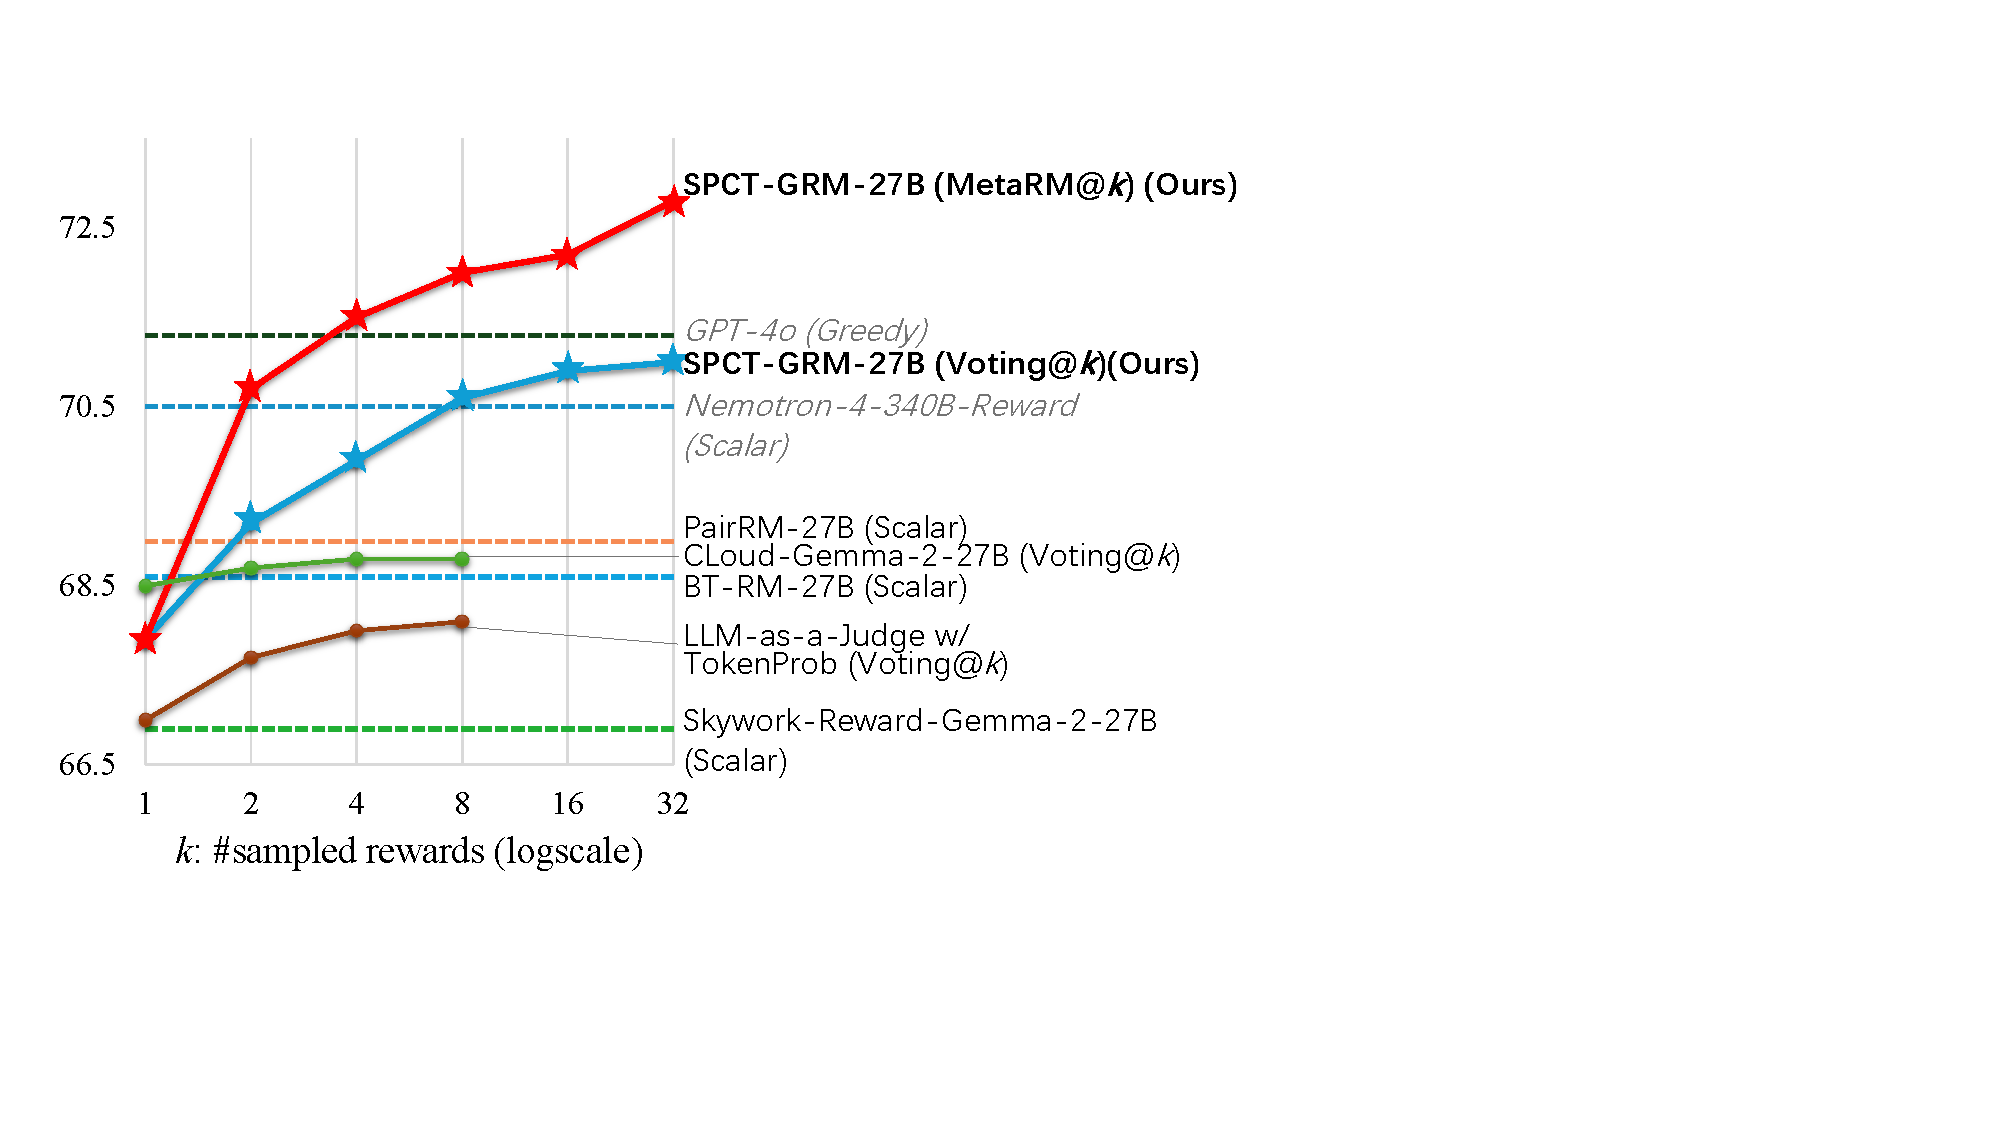
\includegraphics[width=1in,height=1.25in,clip,keepaspectratio]{fig1}}]{Michael Shell}
% Use $\backslash${\tt{begin\{IEEEbiography\}}} and then for the 1st argument use $\backslash${\tt{includegraphics}} to declare and link the author photo.
% Use the author name as the 3rd argument followed by the biography text.
% \end{IEEEbiography}

% \vspace{11pt}

% \bf{If you will not include a photo:}\vspace{-33pt}
% \begin{IEEEbiographynophoto}{John Doe}
% Use $\backslash${\tt{begin\{IEEEbiographynophoto\}}} and the author name as the argument followed by the biography text.
% \end{IEEEbiographynophoto}




\vfill

\end{document}


